\documentclass[11pt,onecolumn,oneside]{article}
\usepackage{epsf,pstricks,pst-grad,color}
\usepackage{graphicx,amssymb,amsmath,makeidx,psfrag,subfigure}
\usepackage{sws,wasysym,epsfig}
\usepackage{a4wide,authda14,graphicx,latexsym,fancyhdr}               
\usepackage{longtable,rotating,latexsym,eso-pic}
\usepackage{eso-pic}
\usepackage[colorlinks=true,citecolor=blue,linkcolor=blue,bookmarks=true,urlcolor=blue,hyperfootnotes=true,plainpages=false,pdfpagelabels=true,breaklinks=true]{hyperref} %create interal an click-on links
\usepackage{breakurl}

\bibliographystyle{authda3}

%\input{abk}
\parindent0em \parskip1.5ex plus0.5ex minus 0.5ex

% -------------------------------------------------------------------

%\geometry{a4paper, left=20 mm, right= 25mm, top=2.0cm, bottom=2.0 cm}

\newcommand\BackgroundPicture{%
   \put(0,-50){
     \parbox[b][\paperheight]{\paperwidth}{
       \vfill
       \centering
%       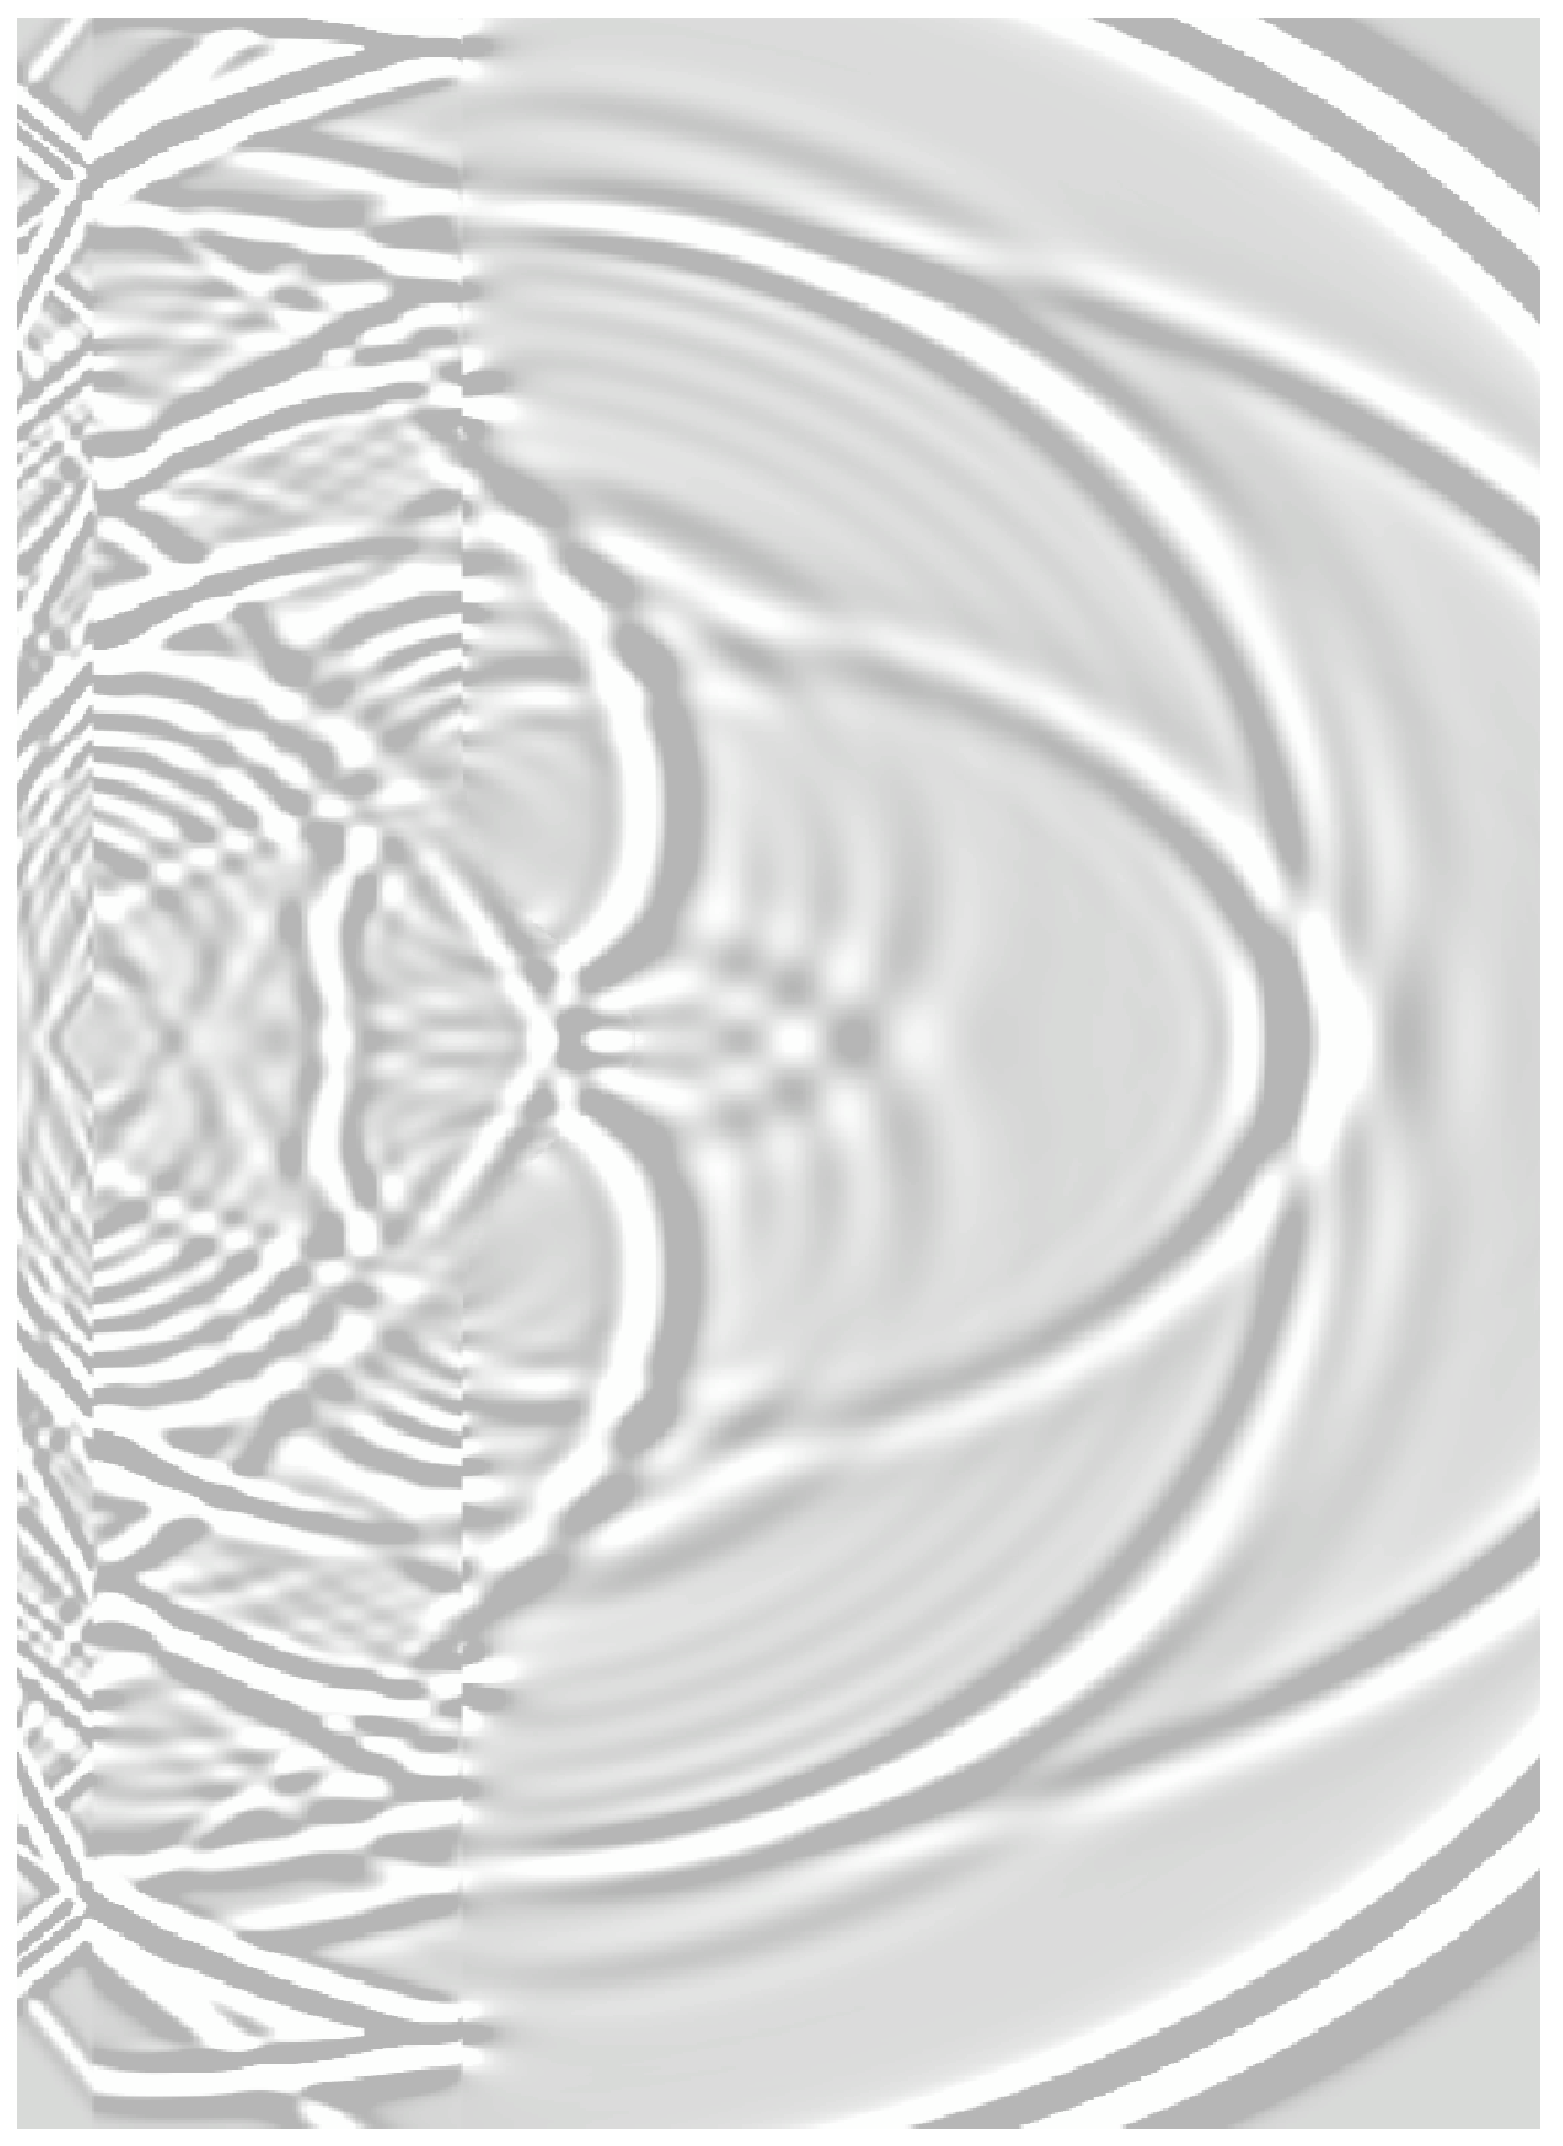
\includegraphics[width=\paperwidth,height=\paperheight,
%                        keepaspectratio]{figures/title_page1.ps}
       
       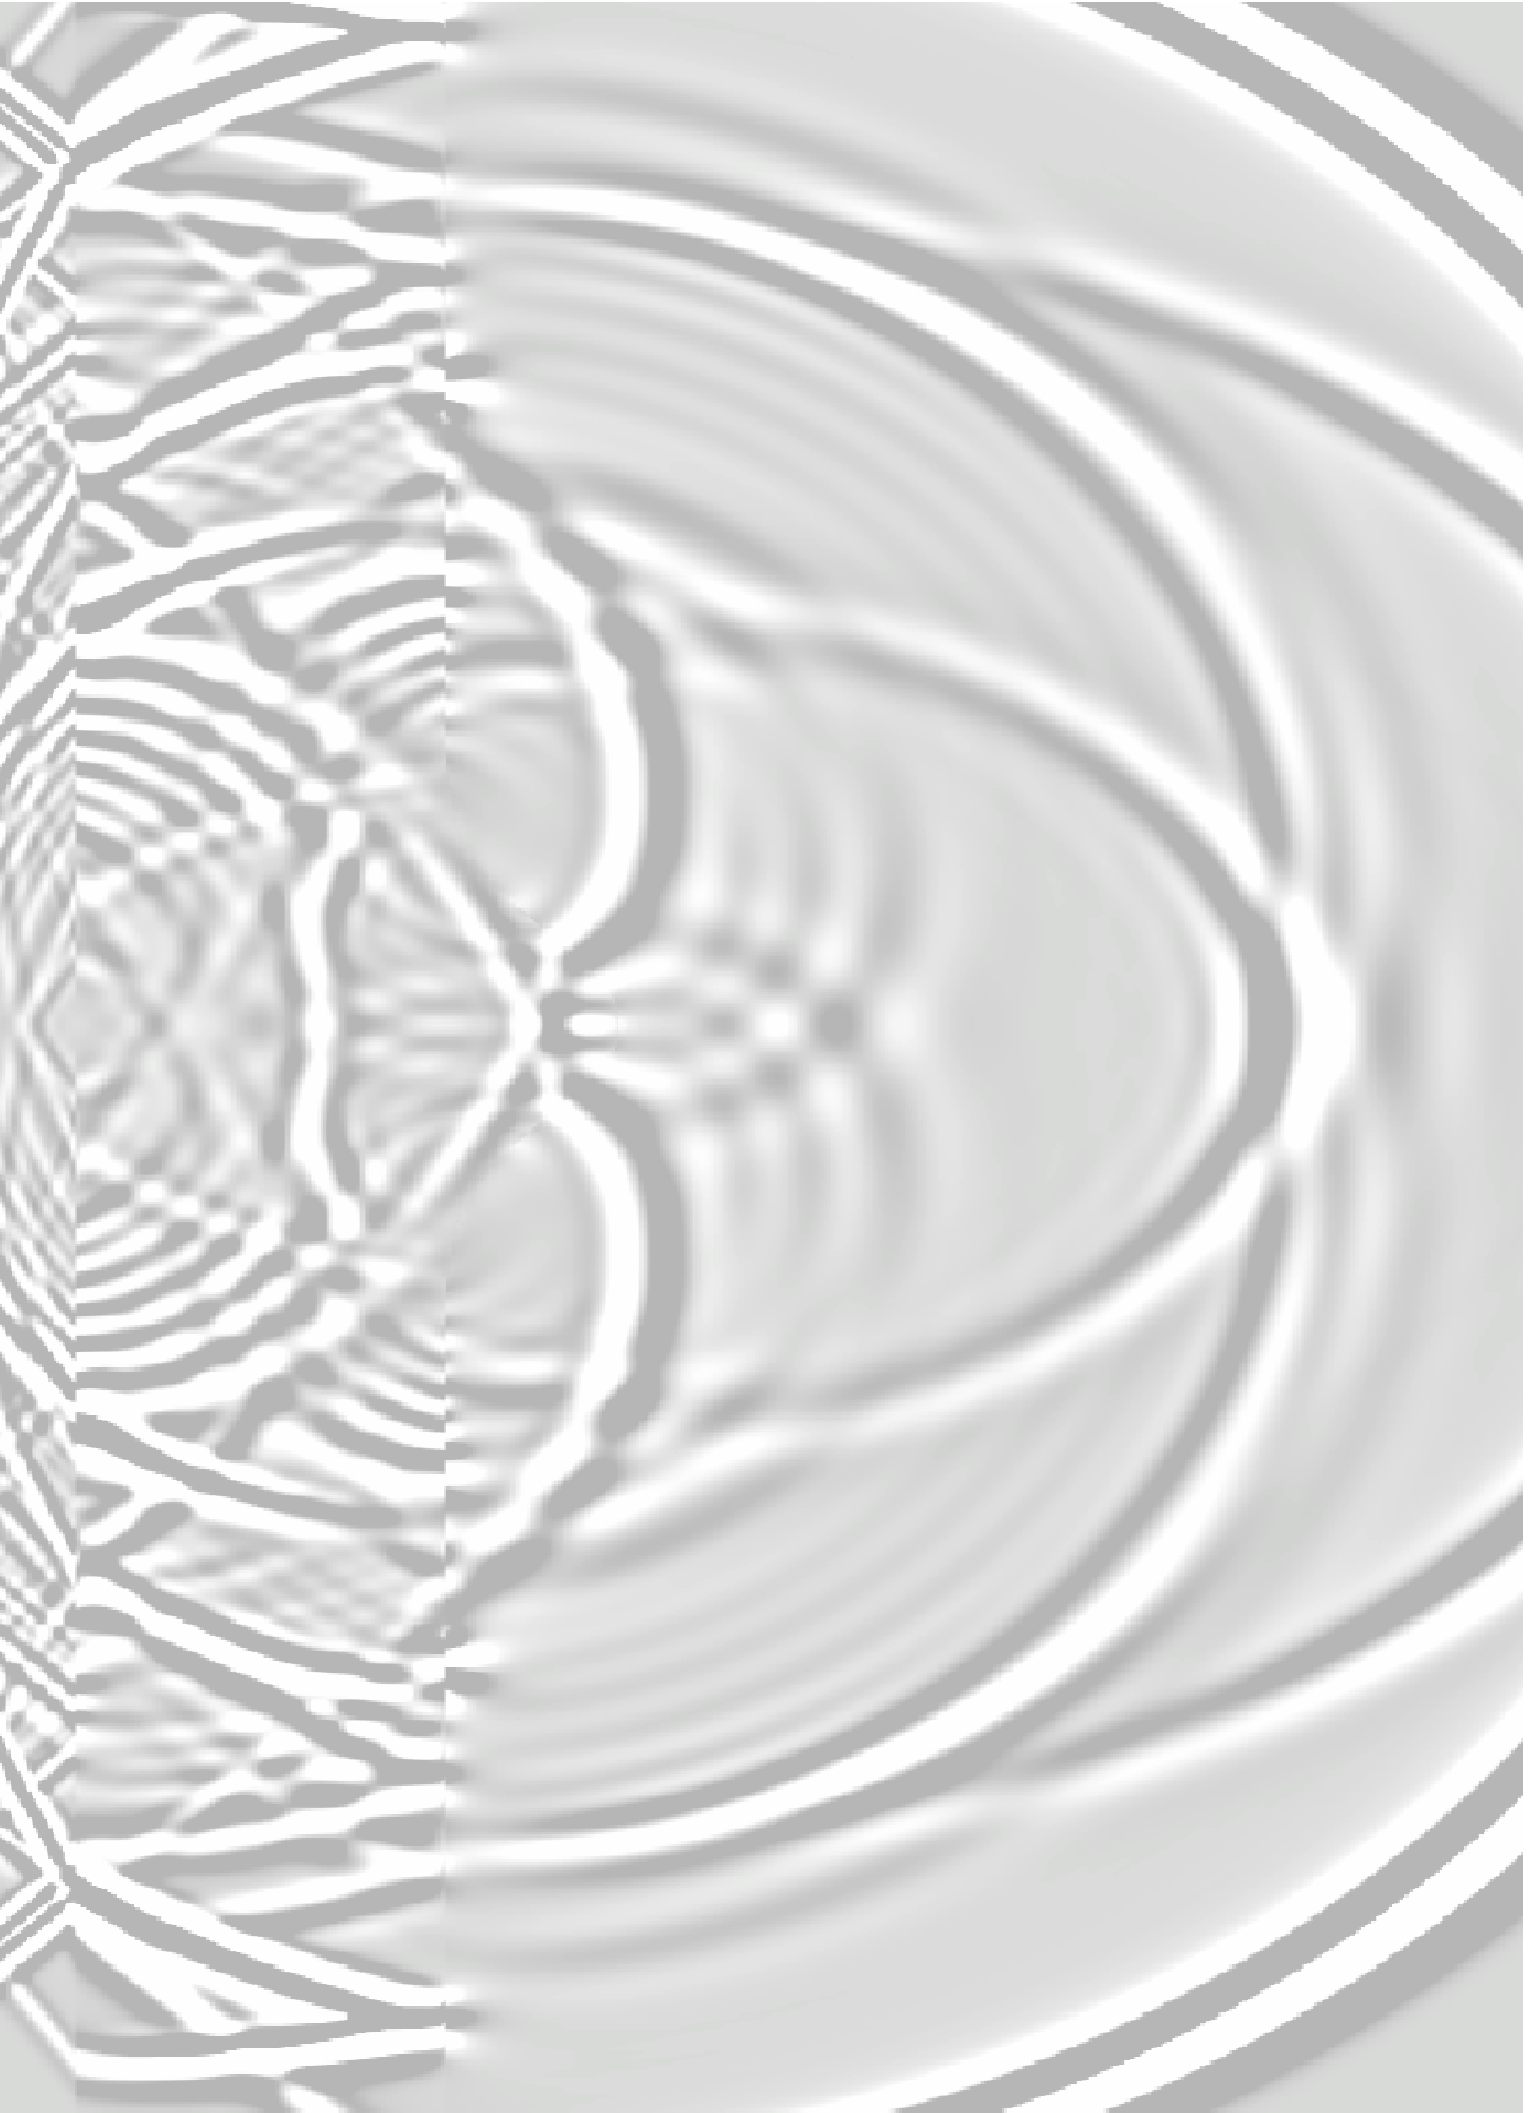
\includegraphics[width=\paperwidth,height=30cm]{figures/title_page1.pdf}
       \vfill
     }}}
% The picture is centered on the page background
% -------------------------------------------------------------------


% add background picture for the titlepage
\AddToShipoutPicture{\BackgroundPicture}

\begin{document}
\thispagestyle{empty}
\newcommand{\Rule}{\rule{\textwidth}{1mm}}
\newtheorem{theorem}{Hypothese}[section]
\begin{center}
\Rule \vspace{5mm}
\sffamily \bfseries \Huge
- SOFI2D - \\ 
seismic modeling with finite differences \\
2D - elastic and viscoelastic version
\vspace{1mm}\Rule\\
\vspace{1 cm}
\Large\emph{Users Guide}\\
\vspace{2 cm}
\large Thomas Bohlen \par
\large Denise De Nil \par
\large Daniel K\"ohn \par
\large Stefan Jetschny\par
\vspace{2 cm}

\small Karlsruhe Institute of Technology\par
\small Department of Physics, Geophysical Institute \par
\small Hertzstrasse 16, 76187 Karlsruhe, Germany \par

\vfill

\includegraphics[height=30mm]{figures/kit_logo_en_4c_positiv.pdf}
\vfill
\large Karlsruhe, \today
\end{center}
\cleardoublepage
\thispagestyle{empty} 
\cleardoublepage
\thispagestyle{empty}
\ClearShipoutPicture

\tableofcontents
\newpage

\section{Requirements}
\label{requirements}

SOFI2D can be generally run under Windows and Linux. You just have to make sure that an MPI implementation (one of the three listed below) is running and a C-Compiler is available. However, the preferred platform is Linux, since most of the large scale cluster computer run under Linux. On our local workstation cluster we use Suse Linux and OpenMPI, most of the test are performed under this system. The following programs should be installed on you machine for a proper run and processing of modeling data. 

\begin{center}
% use packages: array
\begin{small}
\begin{tabular}{lll}
Program & Description & Weblink \\ 
OpenMPI & MPI Implementation & \url{http://www.open-mpi.org} \\
& (for the parallelization) & \\
C-Compiler & the whole code is written in C,& \\
& any C-Compiler should be able & \\
& to compile it & \\
Seismic Un*x & Seismic processing package, & \url{http://www.cwp.mines.edu/cwpcodes} \\
(SU)  & SOFI2D outputs seismic data & \\
& in the SU format & \\
Matlab & Preferred program package for & \url{http://www.mathworks.de} \\
(commercial)& the visualization of snapshots, also  & \\
& useful for the display and & \\
& processing of seismograms & \\
xmovie & Console based movie program, can & usually included in Linux distribution\\
& be used for the quick display & otherwise install from repository\\
& of snapshot data  &
\end{tabular}
\end{small}
\end{center}

\section{Quick guide}\label{qguide}
To compile the program do:

\texttt{cd sofi2D/src}

then

\texttt{make all} or \texttt{make sofi2D}

to compile the program. You may also use the shell script \texttt{compileSOFI2D.sh} located in \texttt{sofi2D/par}. For a successful compiler run you probably need to change the compiler options in \texttt{sofi2D/src/Makefile}. 

To run the program on 8 CPUs do

\texttt{cd sofi2D/par}

\texttt{mpirun -np 8 ../bin/sofi2D ./in\_and\_out/sofi2D.json}


You may also use the shell script \texttt{startSOFI2D.sh} located in \texttt{sofi2D/par} that also writes the screen output to the file \texttt{sofi2D/par/in\_and\_out/sofi2D.jout}.

The modeling parameters are specified in the sofi2D input file \texttt{./in\_and\_out/sofi2D.json}. The parameters should be more or less self-explanatory. The synthetic seismograms and snapshots are written to the files specified in the sofi2D input file.

In the current distribution, the model is generated on the fly by the function sofi2D/src/hh.c. This function generates a homogeneous medium with $v_p$=3500 m/s, $v_s$=2000 m/s, and $\rho$=2000 kg/$\mathrm{m}^3$. Instead, the function readmod.c can be used to read model info from external grid files. See readmod.c for the format of the external files. You can change the function which generates the model grid by switching the READMOD parameter in the sofi2D input file.


\section{License}\label{license}

SOFI2D is free software: you can redistribute it and/or modify it under the terms of the GNU General Public License as published by the Free Software Foundation, version 2.0 of the License only.
 
SOFI2D is distributed in the hope that it will be useful, but WITHOUT ANY WARRANTY; without even the implied warranty of MERCHANTABILITY or FITNESS FOR A PARTICULAR PURPOSE. See the GNU General Public License for more details. You should have received a copy of the GNU General Public License along with SOFI2D. See file COPYING and/or \url{http://www.gnu.org/licenses/gpl-2.0.html}.

The Authors of SOFI2D are listed in file \texttt{AUTHORS}.

\section{Introduction}
In order to extract information about the 2-D structure and composition of the crust from seismic observations, it is necessary to be able to predict how seismic wavefields are affected by complex structures. Since exact analytical solutions to the wave equations do not exist for most subsurface configurations, the solutions can be obtained only  by numerical methods. Various techniques for seismic wave modeling in realistic (complex)  media have been developed. Explicit finite difference methods have been widely used to model seismic wave propagation in 2-D {\em elastic} media, because of their ability to accurately model seismic waves in arbitrary heterogeneous media. The FD software described here is based on the original work of Virieux (1986) and Levander (1988) who both formulated staggered-grid, finite difference scheme based on a system \nocite{levander:88} \nocite{virieux:86} of first-order coupled elastic equations where the variables are stresses  and velocities. This distribution of wavefield and material parameters is referred to a the standard staggered grid (SSG). Robertsson et al. \shortcite{robertsson:94} extended the elastic SSG algorithms of Virieux (1986) and Levander (1988) to the viscoelastic case. To incorporate absorption he applied the ''generalized standard linear solid'' rheological model  (GSLS) which was first proposed by \cite{emmerich:87}.

The main drawback of the FD method is that modeling of realistic models consumes vast quantities of computational resources. Such computational requirements are generally beyond the resources for sequential platforms (single PC or workstation) In recent years it has became feasible to use clusters of workstations or PCs for scientific computing.  FD modeling can benefit from this
technique by using  the message passing interface (MPI) \cite{bohlen:02}. Using the free and portable Message Passing Interface (MPI) the calculations are distributed on PCs or workstations which are connected by an in-house network. By clustering a set of processors, for example PCs running Linux, wall-clock times can be decreased and possible grid sizes  can be increased significantly. 
\clearpage
\section{Equations of motion for an elastic medium}\label{elastic_fd_model} 
The propagation of waves in a general elastic medium\footnote{For equations of motion for an viscoelastic medium and the implementation by finite differences have a look at the Phd thesis of T. Bohlen \cite{bohlen:98}   } can be described by a system of coupled linear partial differential equations. They consist of the equations of motion
\EQ{m:1}{\begin{split}
\varrho \frac{\partial v_i}{\partial t} &= \frac{\partial \sigma_{ij}}{\partial x_j} + f_i\\
\end{split}}   
which simply state that the momentum of the medium, the product of density $\varrho$ and the displacement velocity $v_i$, can be changed by surface forces, described by the stress tensor $\sigma_{ij}$ or body forces $f_i$. These equations describe a general medium, like gas, fluid, solid or plasma. The material specific properties are introduced by additional equations which describe how the medium reacts when a certain force is applied. In the isotropic elastic case this can be described by a linear stress-strain relationship:  
\EQ{m:2}{\begin{split}
\sigma_{ij}&=\lambda \theta \delta_{ij} + 2 \mu \epsilon_{ij}\\
\epsilon_{ij}&=\frac{1}{2}\biggl(\frac{\partial u_i}{\partial x_j}+\frac{\partial u_j}{\partial x_i}\biggr)
\end{split}}   
where $\lambda$ and $\mu$ are the Lam$\rm{\acute{e}}$ parameters, $\epsilon_{ij}$ the strain tensor and $u_i$ the displacement. Using $v_i = \frac{\partial u_i}{\partial t}$, \ER{m:1} and \ER{m:2} can be transformed into a system of second order partial differential equations:
\EQ{2:20}{\begin{split}
\varrho \frac{\partial^2 u_i}{\partial t^2} &= \frac{\partial \sigma_{ij}}{\partial x_j} + f_i\\
\sigma_{ij}&=\lambda \theta \delta_{ij} + 2 \mu \epsilon_{ij}\\
\epsilon_{ij}&=\frac{1}{2}\biggl(\frac{\partial u_i}{\partial x_j}+\frac{\partial u_j}{\partial x_i}\biggr)
\end{split}}
This expression is called {\bf{Stress-Displacement}} formulation. Another common form of the elastic equations of motion can be deduced by taking the time derivative of the stress-strain relationship and the strain tensor in Eq. \ER{2:20}. Since the Lam$\acute{\rm e}$ parameters $\rm{\lambda}$ and $\rm{\mu}$ do not depend on time, Eq. \ER{2:20} can be written as:
\EQ{2:20:1}{\begin{split}
\varrho \frac{\partial v_i}{\partial t} &= \frac{\partial \sigma_{ij}}{\partial x_j} + f_i\\
\frac{\partial \sigma_{ij}}{\partial t} &= \lambda \frac{\partial \theta}{\partial t} \delta_{ij} + 2 \mu \frac{\partial \epsilon_{ij}}{\partial t}\\
\frac{\partial \epsilon_{ij}}{\partial t}&=\frac{1}{2}\biggl(\frac{\partial v_i}{\partial x_j}+\frac{\partial v_j}{\partial x_i}\biggr)
\end{split}}  
This expression is called {\bf{Stress-Velocity}} formulation. For simple cases \ER{2:20} and \ER{2:20:1} can be solved analytically. More complex problems require numerical solutions. One possible approach for a numerical solution is described in the next section.

\section{Solution of the elastic wave equation by finite differences}\label{elastic_FD_Code}

For the numerical solution of the elastic equations of motion, Eqs. \ER{2:20:1} have to be discretized in time and space on a grid. The
particle velocity $\mathbf{v}$, the stresses $\sigma_{ij}$, the p-wave modulus $\pi=\varrho v_p^2=\lambda+2\mu$ and the s-wave modulus $\mu=\varrho v_s^2 $ (with Lam$\acute{\rm e}$ parameters $\rm{\lambda}$ and $\rm{\mu}$) are calculated and 
defined at discrete Cartesian coordinates $x=\rm{i}\; \rm{dh}$, $y=\rm{j}\; \rm{dh}$ and discrete times $t=\rm{n}\; \rm{dt}$. 
$\rm{dh}$ denotes the spatial distance between two adjacent grid points and $\rm{dt}$ the difference between two successive time steps. Therefore every grid point is located in the interval  $i \in \rm{N | [1,NX]}$, $j \in \rm{N | [1,NY]}$ and $\rm{n} \in \rm{N | [1,NT]}$, where
$\rm{NX}$, $\rm{NY}$ and $\rm{NT}$ are the number of discrete spatial grid points and time steps, respectively. Finally the partial derivatives are replaced by {\bf{finite-difference} (FD)} operators. 
Two types of operators can be distinguished, forward and backward operators $\rm{D^+,\;D^-}$. The derivative of a function $y$ with respect to a variable $x$ can be approximated by the following operators:  
\EQ{disc:1}{\begin{split}
\rm{D^+_x} y&= \frac{y{\rm [i+1]} - {\rm my[i]}}{\rm{dh}} \hspace{1 cm} \text{forward operator}\\
\rm{D^-_x} y&= \frac{y{\rm [i]}-y{\rm[i-1]}}{\rm{dh}} \hspace{1 cm} \text{backward operator}\\
\end{split}}\\

 \subsection{Standard staggered grid}
 \label{ssg}
Figure \ref{fig_cell} shows the locations of viscoelastic wavefield parameters and material parameters on the standard staggered grid (SSG). 
On the SSG, different components of one physical parameter are defined at different staggered points. For example, the two different components of the particle velocity (circles in Figure \ref{fig_cell}a) are distributed over two different staggered locations. The different components of the stress tensor (indicated by squares in Figure \ref{fig_cell}a) are distributed over two different locations. The shear modulus $\mu$ and the S-wave attenuation parameter $\tau^s$ \cite{blanch:95,bohlen:02} are required at the locations of shear-stress components. The density $\varrho$ is required
at the locations of particle velocities. These material parameters thus need to be locally averaged, i.e. calculated from neighboring grid points. The averaging of material parameters is critical
for the accuracy at strong discontinuities \cite{zahradnik:93,falk:98,moczo:02}. To obtain stable results, arithmetic averaging  must be used for the density $\varrho$ and attenuation parameter $\tau^s$, and harmonic averaging is required for the shear modulus \cite{fellinger:95,graves:96,falk:98,vossen:02,moczo:02}:

\begin{figure}[tb]
\begin{center}
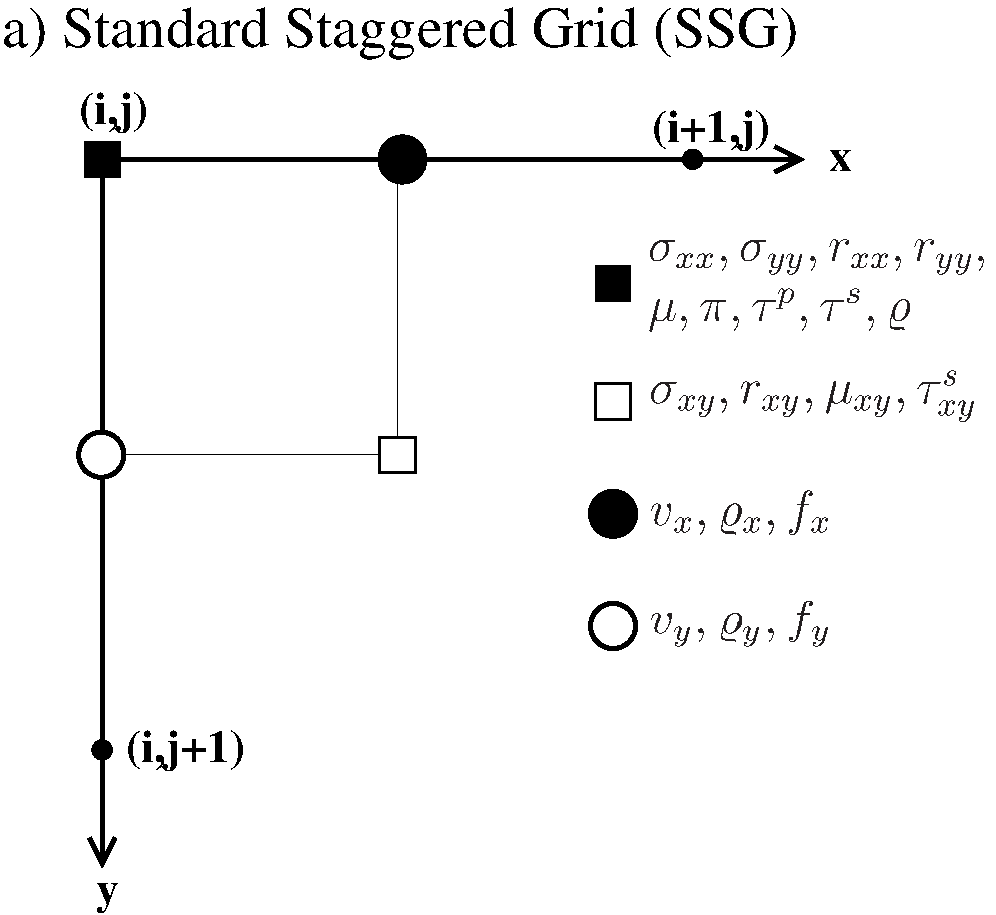
\includegraphics[width=7.4cm,angle=0]{figures/cells_2D_ssg.pdf}
\end{center}
\caption{Locations of wavefield and material parameters in a 2-D finite-difference cell for the Standard Staggered Grid (SSG) \protect\cite{virieux:86,levander:88,robertsson:94}. $\sigma_{ij}$ denote stress components, $r_{ij}$ are the memory variables, $v_i$ are the particle velocities, $f_i$ are the body force components, $\pi$ is the P-wave modulus, $\mu$ is the shear modulus, $\varrho$ denotes density, and $\tau^s$ and $\tau^p$ are the attenuation parameters for P- and S-waves, respectively. $\mu_{xy}$, and $\tau^s_{xy}$,
and $\varrho_x, \varrho_y$ denote averaged material properties for shear modulus, attenuation parameter $\tau^s$, and density, respectively (equation \protect\ref{eq_av_ssg}).}
\label{fig_cell}
\end{figure}


{\small 
\begin{eqnarray}
\varrho_x\rm{[j][i+\frac{1}{2}]}&=&\frac{\varrho\rm{[j][i]}+\varrho\rm{[j][i+1]}}{2}\quad\mbox{,}\nonumber\\
\varrho_y\rm{[j+\frac{1}{2}][i]}&=&\frac{\varrho\rm{[j][i]}+\varrho\rm{[j+1][i]}}{2}\quad\mbox{,}\nonumber\\
\tau^s_{xy}\rm{[j+\frac{1}{2}][i+\frac{1}{2}]}&=&\frac{\tau^s\rm{[j][i]}+\tau^s\rm{[j][i+1]}+\tau^s\rm{[j+1][i+1]}+\tau^s\rm{[j+1][i]}}{4}\mbox{,}\nonumber\\
\mu_{xy}\rm{[j+\frac{1}{2}][i+\frac{1}{2}]}&=&\frac{4}{\mu^{-1}\rm{[j][i]}+\mu^{-1}\rm{[j][i+1]}+\mu^{-1}\rm{[j+1][i+1]}+\mu^{-1}\rm{[j+1][i]}}\mbox{.}\nonumber\\
\label{eq_av_ssg}
\end{eqnarray}}
%This averaging procedure satisfies the condition of traction continuity across the interface between two media on standard staggered grids \cite{moczo:02}.
%Harmonic averaging of the shear modulus $\mu$  yields higher
%accuracy than arithmetic averaging for modeling Scholte waves propagating along
%fluid-solid interfaces  \cite{falk:98}.
%Our numerical tests show that arithmetic averaging of the shear modulus across free surfaces leads to instabilities. Harmonic averaging produces stable simulations. 
%For the SSG the location of the free surface is  defined by the plane going through the staggered position of the particle velocity $v_y$ and shear stress $\sigma_{xy}$ (Figure \ref{fig_cell}a). As a consequence the computation of the curl (S-wave component) and divergence (P-wave component) of the particle velocity wavefield is not accurate at the free surface because $v_x$ is located outside and $v_y$ inside the medium.
  
%The determination of the actual location of an interface between two media on the SSG is not a trivial task. Only in the case that interfaces are aligned with the grid the interface location can be determined. On curved interfaces, however, the interface location cannot be determined exactly due to the staggered grid representation of the model. 

\subsection{Discretization of the wave equation}

The discretization of the linear stress strain relationship in \ER{2:20:1} at time step n leads to the following system of equations :
\EQ{cart_dis:1}{\begin{split}
v_{xx}{\rm [j][i]} & \approx \frac{v_x {\rm [j][i+\frac{1}{2}]}-v_x\rm{[j][i-\frac{1}{2}]}}{{\rm dh}}\\
v_{yy}{\rm [j][i]} & \approx \frac{v_y {\rm [j+\frac{1}{2}][i]}-v_y\rm{[j-\frac{1}{2}][i]}}{{\rm dh}}\\
v_{yx}{\rm [j+\frac{1}{2}][i+\frac{1}{2}]} & \approx \frac{v_y {\rm [j+\frac{1}{2}][i+1]}-v_y {\rm [j+\frac{1}{2}][i]}}{\rm{dh}}\\
v_{xy}{\rm [j+\frac{1}{2}][i+\frac{1}{2}]} & \approx \frac{v_x {\rm [j+1][i+\frac{1}{2}]}-v_x {\rm [j][i+\frac{1}{2}]}}{\rm{dh}}\\
\sigma_{xy}^{\rm n} {\rm [j+\frac{1}{2}][i+\frac{1}{2}]}&=\sigma_{xy}^{\rm n-1} {\rm [j+\frac{1}{2}][i+\frac{1}{2}]} + {\rm dt}\cdot\mu_{xy} {\rm [j+\frac{1}{2}][i+\frac{1}{2}]}\biggl(v_{xy} {\rm [j+\frac{1}{2}][i+\frac{1}{2}]} + v_{yx} {\rm [j+\frac{1}{2}][i+\frac{1}{2}]}\biggr)\\
\sigma_{xx}^{\rm n} {\rm [j][i]}&=\sigma_{xx}^{\rm n-1} {\rm [j][i]} + {\rm dt}\cdot\pi {\rm [j][i]}\cdot\biggl(v_{xx} {\rm [j][i]} - v_{yy} {\rm [j][i]} \biggr) - 2 \cdot {\rm dt} \cdot \mu {\rm [j][i]} \cdot v_{xx} {\rm [j][i]}\\
\sigma_{yy}^{\rm n} {\rm [j][i]}&=\sigma_{yy}^{\rm n-1} {\rm [j][i]} + {\rm dt}\cdot\pi {\rm [j][i]}\cdot\biggl(v_{xx} {\rm [j][i]} - v_{yy} {\rm [j][i]} \biggr) - 2 \cdot {\rm dt} \cdot \mu {\rm [j][i]} \cdot v_{yy} {\rm [j][i]}\\
\end{split}} 
 
The discretization of the momentum equation in \ER{2:20:1} leads to the following system of equations:
\EQ{cart_dis:2}{\begin{split}
vtt_x {\rm [j][i+\frac{1}{2}]} &= \biggl(\sigma_{xx} \rm{[j][i+1]} - \sigma_{xx}\rm{[j][i]} + \sigma_{xy}\rm{[j+\frac{1}{2}][i]} - \sigma_{xy}\rm{[j-\frac{1}{2}][i]} \biggr)\\
vtt_y {\rm [j+\frac{1}{2}][i]} &= \biggl(\sigma_{xy}\rm{[j][i+\frac{1}{2}]} - \sigma_{xy} {\rm [j][i-\frac{1}{2}]} + \sigma_{yy} {\rm [j+1][i]} - \sigma_{yy} {\rm [j][i]} \biggr)\\
v_x^{\rm n} {\rm [j][i+\frac{1}{2}]}&= v_x^{\rm n-1} {\rm [j][i+\frac{1}{2}]} + \frac{{\rm dt}}{{\rm dh}\cdot\varrho_x {\rm [j][i+\frac{1}{2}]}}\cdot vtt_x {\rm [j][i+\frac{1}{2}]}\\
v_y^{\rm n} {\rm [j+\frac{1}{2}][i]}&= v_y^{\rm n-1} {\rm [j+\frac{1}{2}][i]} + \frac{{\rm dt}}{{\rm dh}\cdot\varrho_y {\rm [j+\frac{1}{2}][i]}}\cdot vtt_y {\rm [j+\frac{1}{2}][i]}\\
\end{split}} 


\subsection{Accuracy of FD operators}
The derivation of the FD operators in the last section was a simple replacement of the partial derivatives by finite differences. In the following more systematic approach, the first derivative of a variable f at a grid point i is estimated by a Taylor series expansion \cite{jastram:92a}:
\EQ{op_acc:1}{\begin{split}
\rm{(2k-1)\frac{\partial f}{\partial x}\biggr|_i}&\rm{=\frac{1}{\rm{dh}}(f_{i+(k-1/2)}-f_{i-(k-1/2)})}\\
&\rm{+\frac{1}{\rm{dh}}\sum_{l=2}^N \frac{((k-\frac{1}{2}) \rm{dh})^{2l-1}}{(2l-1)!}\frac{\partial^{(2l-1)}f}{\partial
x^{(2l-1)}}\biggr|_i+{\mathcal{O}}(\rm{dh})^{2N}} \notag
\end{split}}
For an operator with length 2N, N equations are added with a weight $\rm{\beta_k}$:
\EQ{op_acc:2}{\begin{split}
\rm{[\sum_{k=1}^{N} \beta_k (2k-1)]\frac{\partial f}{\partial x}\biggr|_i}&\rm{=\frac{1}{\rm{dh}} \sum_{k=1}^{N} \beta_k (f_{i+(k-1/2)}-f_{i-(k-1/2)})}\\
&\rm{+\frac{1}{\rm{dh}}\sum_{k=1}^{N} \sum_{l=2}^N \beta_k \frac{((k-\frac{1}{2}) \rm{dh})^{2l-1}}{(2l-1)!}\frac{\partial^{(2l-1)}f}{\partial
x^{(2l-1)}}\biggr|_i+{\mathcal{O}}(\rm{dh})^{2N}}
\end{split}}
The case N=1 leads to the FD operator derived in the last section, which has a length of 2N=2. The Taylor series is truncated after the first term ($\rm{{\mathcal{O}}(\rm{dh})^{2}}$). 
Therefore this operator is called {\bf{2nd order FD operator}} which refers to the truncation error of the Taylor series and not to the order of the approximated derivative.
To understand equation \ER{op_acc:2} better, we estimate a {\bf{4th order FD operator}}. This operator has the length 2N = 4 or N=2. The sums in Eq. \ER{op_acc:2} lead to:
\EQ{op_acc:3}{\begin{split}
\rm{(\beta_1+3 \beta_2) \frac{\partial f}{\partial x}\biggr|_i}&\rm{=\frac{1}{\rm{dh}}(\beta_1(f_{i+1/2}-f_{i-1/2})+\beta_2(f_{i+3/2}-f_{i-3/2}))}\\
&\rm{+\frac{\rm{dh}^3}{\rm{dh}}\biggl[\beta_1\frac{1}{8 \cdot 3!}+\beta_2\frac{27}{8 \cdot 3!}\biggr]\frac{\partial^3 f}{\partial x^3}\biggr|_i}
\end{split}}
The weights $\rm{\beta_k}$ can be calculated by the following approach: 
The factor in front of the partial derivative on the LHS of Eq. \ER{op_acc:3} should equal 1, therefore
\EQ{op_acc:4}{\rm{(\beta_1+3\beta_2)=1 \notag.}}
The coefficients in front of $\rm{\frac{\partial^3 f}{\partial x^3}\biggr|_i}$ on the RHS of Eq. \ER{op_acc:3} should vanish:
\EQ{op_acc:5}{\rm{(\beta_1+27\beta_2)=0 \notag.}}
The weights $\rm{\beta_k}$ can be estimated by solving the matrix equation:
\EQ{op_acc:6}{
\rm{\left(
\begin{array}{ll}
1 & 3 \\
1 & 27 \\
\end{array}
\right)\cdot \hspace{0.2 cm}
\left(
\begin{array}{l}
\beta_1 \\
\beta_2 \\
\end{array}
\right)
=
\left(
\begin{array}{l}
1 \\
0 \\
\end{array}
\right) \notag}
}
The resulting coefficients are $\rm{\beta_1=9/8}$ and $\rm{\beta_2=-1/24}$. Therefore the 4th order backward- and forward operators are:
\EQ{op_acc:7}{\begin{split}
\rm{\frac{\partial f}{\partial x}\biggr|_{i+1/2}}&\rm{=\frac{1}{\rm{dh}}[\beta_1 (f_{i+1}-f_i)+\beta_2 (f_{i+2}-f_{i-1})] \hspace{1 cm} \text{forward operator}}\\
\rm{\frac{\partial f}{\partial x}\biggr|_{i-1/2}}&\rm{=\frac{1}{\rm{dh}}[\beta_1 (f_{i}-f_{i-1})+\beta_2 (f_{i+1}-f_{i-2})] \hspace{1 cm} \text{backward operator}}\\
\end{split}}
The coefficients $\rm{\beta_i}$ in the FD operator are called {\bf{Taylor coefficients}}. 
%Generally the Taylor coefficients can be calculated using the recursive equation (\cite{liu:2009})
%\EQ{op_acc:8}{\begin{split}
%\rm{\beta_i}&\rm{=\frac{(-1)^{i+1}}{i^2}\prod_{1 \le n \le 2N, n \ne i} \biggl|\frac{n^2-1}{n^2-i^2}\biggr| \; (i=1,2,...,2N).}\\
%\end{split}}
The accuracy of higher order FD operators can be improved by seeking for FD coefficients $\rm{\beta_k}$ that approximate the first derivative in a certain frequency range \cite{holberg:87}. These numerically optimized coefficients are called {\bf{Holberg coefficients}}.

\subsection{Adams-Bashforth fourth-order accurate time integrators}
To improve the precision of the temporal discretization the Adams-Bashforth fourth-order accurate time integrator can be used. 
The staggered Adams-Bashforth method (ABS) is a multi-step method that uses previously calculated wavefields to increase the accuracy order in time.\\
In \cite{bohlen2015higher2} and \cite{bohlen2015higher} we give a detailed study of the performance of the ABS method in 1-D and 3-D. The analysis shows that the numerical dispersion is much lower than that of the widely used second-order leapfrog method. However numerical dissipation is introduced by the ABS method. In simulation experiments the convincing improvements of accuracy of the fourth-order ABS method is verified. For instance, in a realistic elastic 3-D scenario the computing time reduces by a factor of approximately 2.2, whereas the memory requirements increase by approximately the same factor.\\
The ABS method thus provides an alternative strategy to increase the time accuracy by investing computer memory instead of computing time.\\

In the following we provide an extract of \cite{bohlen2015higher2} to demonstrate the underlying theory. Additionally seismograms of different temporal orders of accuracy and an analysis of the numerical simulation error are shown.\\ 
In SOFI2D only a fourth-order accurate Adams-Bashforth time integrator is implemented, due to the superior performance over third-order.
\subsubsection{Theory}
For the sake of simplicity we illustrate the staggered Adams-Bashforth method (ABS-method) using the 1-D acoustic wave equation in velocity-stress formulation
\begin{eqnarray}
\frac{\partial p(x,t)}{\partial t}&=& - \pi (x) \frac{\partial v(x,t)}{\partial x}  \notag \\
\frac{\partial v(x,t)}{\partial t}&=& -\rho^{-1}(x) \frac{\partial p(x,t)}{\partial x}
\label{waveequation}
\end{eqnarray}
The wavefield variables are the pressure $p(x,t)$ and the particle velocity $v(x,t)$. The material is described by the P-wave modulus $\pi (x)$ and the mass density $\rho(x)$. For simplicity we omit the temporal ($t$) and spatial dependencies ($x$)  in the following.

Using the conventional second order staggered grid approximation to the first order time derivative we obtain
\begin{eqnarray}
\frac{p |^{n+1/2}-p|^{n-1/2}}{\Delta t}&=& - \pi \frac{\partial v}{\partial x}\bigg |^n  + \mathcal{O}(\Delta t^2) \nonumber \\ 
\frac{v|^n-v|^{n-1}}{\Delta t}&=& -\rho^{-1} \frac{\partial p}{\partial x}\bigg |^{(n-1/2)} + \mathcal{O}(\Delta t^2)
\label{2ndorder}
\end{eqnarray}

This results in the conventional explicit second order accurate time-stepping (leapfrog) scheme
\begin{eqnarray}
p|^{n+1/2}&=&p|^{n-1/2} - \Delta t \pi \frac{\partial v}{\partial x}\bigg |^n  + \mathcal{O}(\Delta t^2) \nonumber \\
v|^n&=&v|^{n-1} -\Delta t \rho^{-1} \frac{\partial p}{\partial x}\bigg |^{(n-1/2)}  + \mathcal{O}(\Delta t^2)
\label{2ndorderexplicit}
\end{eqnarray}
which requires no additional storage of the wavefield variables $p$ and $v$. 

With the ABS-method the order of the temporal integration  can be increased by using previous time levels of the right hand sides of equation \ref{2ndorder} \cite{ghrist2000staggered}.
The ABS-method thus requires the storage of previous time levels of spatial derivatives of the pressure $p$ and particle velocity $v$. The time update for the ABS-method thus reads
\begin{eqnarray}
p|^{n+1/2}&=&p|^{n-1/2} - \Delta t \pi \sum_{k=0}^{M-1} a_k \frac{\partial v}{\partial x}\bigg |^{n-k}   + \mathcal{O}(\Delta t^M) \nonumber \\
v|^n&=&v|^{n-1} -\Delta t \rho^{-1}  \sum_{k=0}^{M-1} a_k  \frac{\partial p}{\partial x}\bigg |^{(n-1/2-k)}  + \mathcal{O}(\Delta t^M)
\label{absmethod}
\end{eqnarray}
The weights for the time accuracy orders $M=2,3,4$ are given in Table \ref{absweights}. 

\begin{table}[ht]
\begin{center}
\begin{tabular}{|c|c|c|c|c|}\hline
$M$ & $a_0$ & $a_1$ & $a_2$ & $a_3$  \\ \hline
2 & 1             &  0           &  0           &     0   \\
3 &  25/24     &  -1/12         & 1/24   & 0   \\
4 & 13/12      &  -5/24      &  1/6       &  -1/24     \\ \hline
\end{tabular}
\end{center}
\caption{\label{absweights}Weights used for the summation of previous time levels in the Adams-Bashforth method \protect\cite{ghrist2000staggered}.}
\end{table}
\newpage
\subsubsection{Accuracy in 1-D}
We first compare seismograms calculated with the 1-D ABS-method using equations \ref{absmethod} for different orders of accuracy in time ($M$). We use a 1-D homogeneous acoustic 
medium with a wave velocity of $c=3500$\,m/s and constant density of $\rho=2000$\,kg/m$^3$ . The source signal is a Ricker signal with a center frequency of 600\,Hz. We choose a large source-receiver distance of 120 dominant wavelength to emphasize the effects of numerical dispersion and numerical dissipation in the synthetic seismograms. The spatial derivatives are
computed with high accuracy using a centered staggered FD stencil of 8th order accuracy.  The spatial grid spacing is held constant at $\Delta x=0.4$\,m corresponding to approximately 14 grid points per dominant wavelength. Discrepancies to the analytical solution (time-shifted Ricker signal) are thus mainly caused by the chosen time step interval $\Delta t$ and the order of the temporal discretization ($M=2,3,4$). The numerical results for Courant numbers $r=c \Delta t/\Delta x=0.4, 0.2, 0.1$ and temporal orders of accuracy $M=2, 3, 4$ are compared with the analytical solution in Figure \ref{fig_1dfdseis}.  For a large Courant number of $r=0.4$ (corresponding to a large time step interval) and second order approximation of the time derivative ($M=2$) we can observe a large time dispersion error causing a leading phase with high amplitude (Figure \ref{fig_1dfdseis}, top-left). Figure  \ref{fig_1dfdseis} compares two ways to reduce this time discretization error. The conventional way is to  stay with the given temporal accuracy order (typically $M=2$) and then reduce the time step interval, i.e. Courant number. The resulting waveforms are shown in the rows of Figure  \ref{fig_1dfdseis}.
Reducing the Courant number (time step interval) will increase the computation time proportional to $1/r$.  The alternative  way proposed in this study is to increase the order of the temporal discretization with the ABS-method which requires to store $M-1$ previously calculated spatial derivates of wavefields. The resulting waveforms are shown in the columns of  Figure  \ref{fig_1dfdseis}. \\ \\

In Figure \ref{fig_1dfdseis} we see that the simulation accuracy increases with decreasing Courant number and increasing accuracy order.  In order to quantify the corresponding numerical simulation error we calculated the normalized L2-misfit between the numerical and analytical solution for different Courant numbers and accuracy orders 
$M = 2, 3, 4$. 
In Figure \ref{fig_L2} we plot the normalized L2-misfit over the number of time steps $NT=T/\Delta t=T c/(r \Delta x)$ where the propagation time of waves is held fixed at $T=0.24$\,s. We can observe the expected higher order reduction of the simulation accuracy which reduces proportional to $\Delta t^{M}$ or $NT^{-M}$. For a given accuracy level of $E=0.1\%$ (horizontal line in Figure \ref{fig_L2}) the required numbers of time steps are 39233, 13938, and 8704 for $M=2,M=3$ and $M=4$, respectively. The number of time steps thus reduces  to $36\%$  and $22\%$  when we increase the temporal order from $M=2$ to  $M=3$ and $M=4$, respectively (Figure  \ref{fig_L2} ). The ABS methods thus allows to significantly decrease the number of time steps and thus to save computing time. \\ \\
\begin{figure*}[!h]
\begin{center}
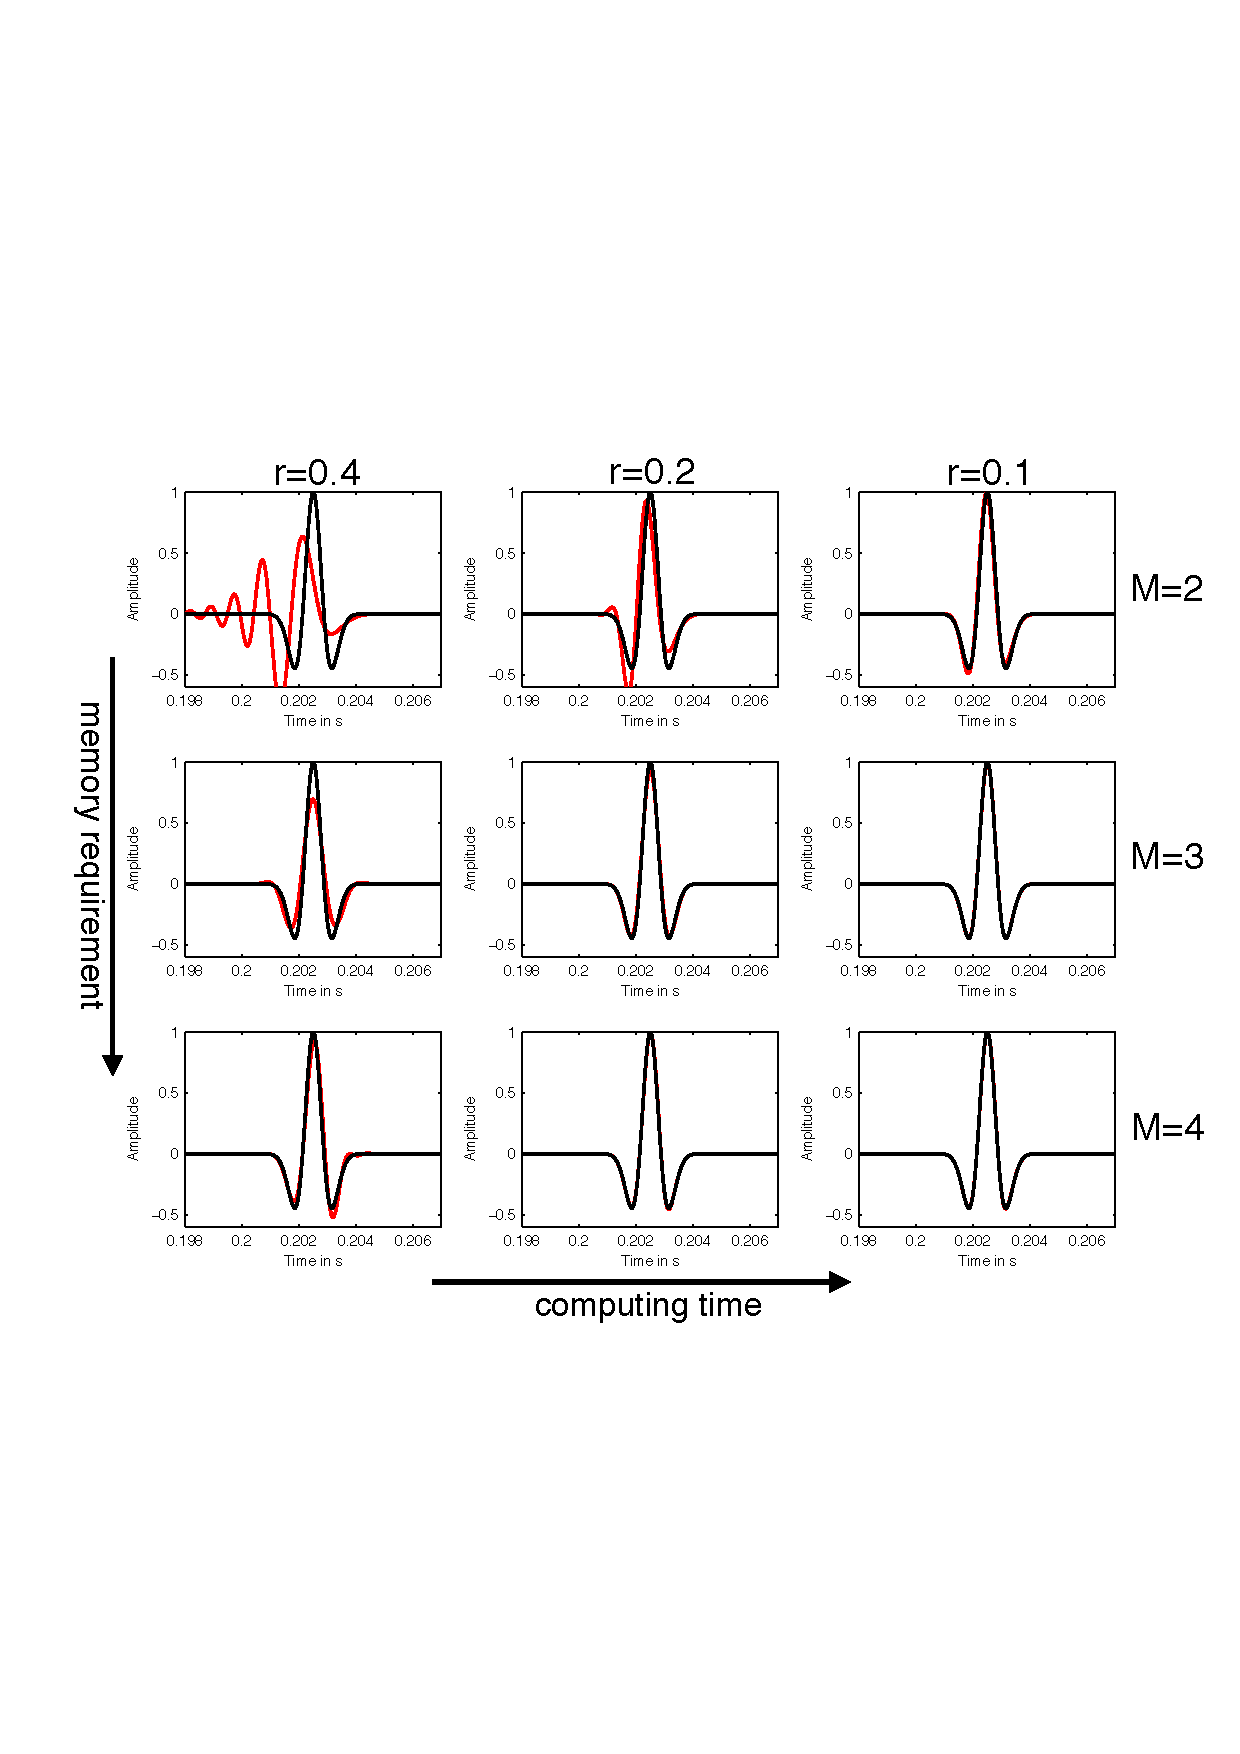
\includegraphics[width=\textwidth]{figures/seismo.pdf}
\caption{Seismograms (red lines) calculated for the 1-D case for different Courant numbers $r$ and accuracy orders $M$. $M=2$ corresponds to the classical second order leapfrog scheme (equations \ref{2ndorder}). $M=3,4$ correspond to the multi-step ABS method (equations \ref{absmethod}). The analytical solution is plotted as a black line. }
\label{fig_1dfdseis}
\end{center}
\end{figure*}
\begin{figure}[h]
\begin{center}
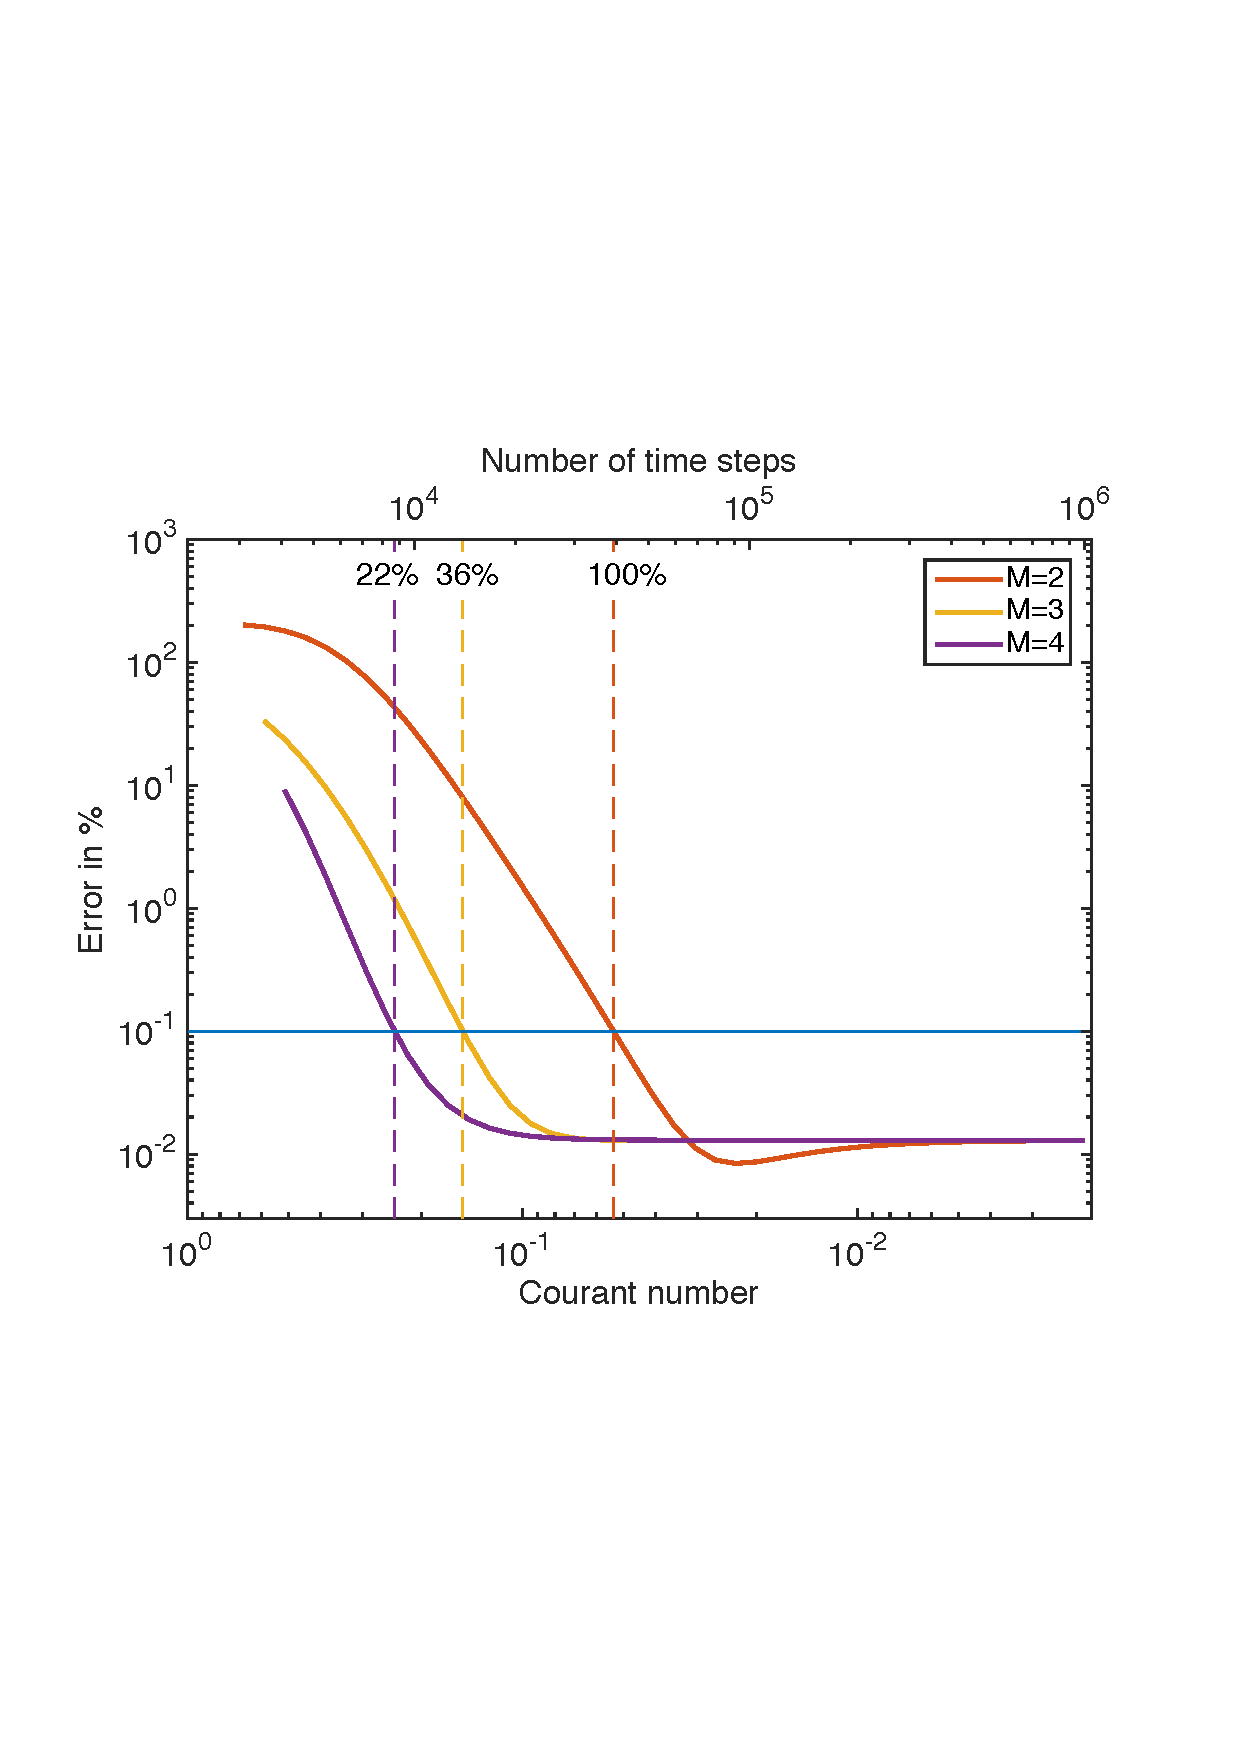
\includegraphics[scale=0.7]{figures/error_1D_courant}
\caption{Relative error of 1-D simulations (Figure \ref{fig_1dfdseis}). 
The normalized L2 norm is plotted over the required number of time steps ($NT$). The temporal accuracy orders are $M=2,3,4$. The spatial accuracy is fixed at order $N=8$. 
The number of time steps to achieve a given accuracy of $E=0.01\%$ (horizontal line) reduce to $36\%$ and $22\%$ for the temporal orders $M=3$ and $M=4$, respectively. 
For large $NT$ (small time step intervals) the error converges to the fixed error of the spatial discretization. }
\label{fig_L2}
\end{center}
\end{figure}
\newpage
\subsection{Free Surface}
The interface between the elastic medium and air at the surface is very important when trying to model surface waves or multiple reflections
in a marine environment. Since all stresses in the normal direction at this interface vanish
\EQ{free:1}{\sigma_{xy} = \sigma_{yy}  = 0.0}
this boundary condition is called (stress) {\bf{free surface}}.
Two types of implementations are common. In the implicit defintion of the free surface, a small layer with the acoustic parameters of air
($V_p=300\;m/s$, $V_s=0.0\;m/s$, $\varrho=1.25\;kg/m^3$) is placed on top of the model. One advantage of the implicit definition
of the free surface is the easy implementation of topography on the FD grid, however to get accurate results for surface waves or multiples,
this approach requires a fine spatial sampling of the FD grid near the free surface. An explicit free surface can be implemented by using
the mirroring technique by Levander, which leads to stable and accurate solutions for plain interfaces \cite{levander:88}, \cite{robertsson:95}. If the planar free surface is located at grid point $\rm{j=h}$, the stress at this point is set to zero and the stresses below the free surface are mirrored with an inverse sign:
\EQ{free:2}{\begin{split}
\sigma_{yy}\rm{[h][i]} &= 0 \\
\sigma_{yy}\rm{[h-1][i]} &= - \sigma_{yy}\rm{[h+1][i]}\\
\sigma_{xy}\rm{[h-\frac{1}{2}][i+\frac{1}{2}]} &= - \sigma_{xy}\rm{[h+\frac{1}{2}][i+\frac{1}{2}]}\\
\sigma_{xy}\rm{[h-\frac{3}{2}][i+\frac{1}{2}]} &= - \sigma_{xy}\rm{[h+\frac{3}{2}][i+\frac{1}{2}]}\\
\end{split}}
When updating the stress component 
\EQ{sxx}{
\sigma_{xx}={\rm dt}\, \pi ( v_{xx} + v_{yy} ) -2 {\rm dt}\, \mu\, v_{yy}
}
 at the free surface only horizontal particle velocities should be used because vertical derivatives over the free surface lead to instabilities (\cite{levander:88}). The vertical derivative of the y-velocity $v_{yy}$ can be replaced by using the boundary condition at the free surface:
\EQ{free:3}{\begin{split}
\sigma_{yy} &= {\rm dt}\, \pi\left(v_{xx} + v_{yy}\right)  - 2 {\rm dt}\, \mu\, v_{xx} = 0 \\
v_{yy} &= - \frac{(\pi-2\mu )}{\pi} v_{xx} \\
\end{split}}
Therefore equation \ER{sxx}  can be written as
\EQ{free:4}{\begin{split}
\sigma_{xx}={\rm dt}\left(4\mu -\frac{(2\mu)^2}{\pi} \right) v_{xx}
\end{split}}


\subsection{Absorbing Boundary Conditions}
Due to limited computational resources, the FD grid has to be as small as possible. To model problems with an infinite extension in different directions, e.g. a full or half-space problem,  an artificial absorbing boundary condition has to be applied. A very effective way to damp the waves near the boundaries are {\bf{Perfectly Matched Layers (PMLs)}}. This can be achieved by a coordinate stretch of the wave equations in the
frequency domain \cite{komatitsch:07}. The coordinate stretch creates exponentially decaying plane wave solutions in the absorbing boundary frame. The PML's are only
reflectionless if the exact wave equation is solved. As soon as the problem is discretized (for example using finite differences) you are solving an approximate wave equation and
the analytical perfection of the PML is no longer valid. In sofi2D a damping profile $d_x$ after \cite{collino2001application} is implemented:

\begin{equation}
d_x(x)=d_0\left( \frac{x}{L}\right) ^n,
\end{equation}
where $L$ denotes the width of the absorbing frame and $d_0$ is a function of the theoretical reflection coefficient $R$:

\begin{equation}
d_0=-\left( n+1\right) V_{PML}\frac{log(R)}{2L},
\end{equation}
where $V_{PML}$ denotes the typical P-wave velocity of the medium in the absorbing boundary frame. A reflection coefficient of $R=1 \times 10^{-4}$ is assumed.
The PMLs are damping the seismic waves by a factor 5-10 more effective than the conventional absorbing boundary frame.
\clearpage
\section{Numerical Artefacts and Instabilities}\label{num_instab}
To avoid numerical artefacts and instabilities during a FD modeling run, a spatial and temporal sampling condition for the wavefield has to be satisfied. These will be discussed in the following two sections. 

\subsection{Grid Dispersion}\label{grid-dispersion}
The first question when building a FD model is: What is the maximum spatial grid point distance dh, for a correct sampling of the wavefield? To answer this question we take a look at this simple example: The particle displacement in x-direction is defined by a sine function:
\EQ{grid_disp:1}{v_x=\sin\biggl(2 \pi \frac{x}{\rm{\lambda}}\biggr),}
where $\rm{\lambda}$ denotes the wavelength. When calculating the derivation of this function analytically at $x=0$ and setting $\rm{\lambda}=1\;\rm{m}$ we get:
\EQ{grid_disp:2}{\frac{d v_x}{d x}\biggl|_{x=0}=\frac{2 \pi}{\rm{\lambda}} \cos\biggl(2 \pi \frac{x}{\rm{\lambda}}\biggr)\biggl|_{x=0}=2 \pi.}
In the next step the derivation is approximated numerically by a staggered 2nd order finite-difference operator:
\EQ{grid_disp:3}{\frac{d v_x}{d x}\biggl|_{x=0} \approx \frac{v_x(x+\frac{1}{2}\Delta x)-v_x(x-\frac{1}{2}\Delta x)}{\Delta x}\biggl|_{x=0}=\frac{\sin \biggl(\frac{2 \pi (\frac{1}{2}{\rm dx})}{\rm{\lambda}} \biggr)-\sin \biggl(\frac{2 \pi (\frac{1}{2}{\rm dx})}{\rm{\lambda}} \biggr)}{\Delta x}.}
Using the Nyquist-Shannon sampling theorem it should be sufficient to sample the wavefield with $\Delta x = \rm{\lambda}/2$. In table \ref{grid_disp.1} the
numerical solutions of eq. \ER{grid_disp:3} and the analytical solution \ER{grid_disp:2} are compared for different sample intervals 
$\Delta x = \rm{\lambda} /n$, where n is the number of gridpoints per wavelength. For the case n=2, which corresponds to the Nyquist-Shannon theorem, the
numerical solution is $\frac{d v_x}{d x}|_{x=0}=4.0$, which is not equal with the analytical solution $2 \pi$. A refinement of the spatial
sampling of the wavefield results in an improvement of the finite difference solution. For $\rm n=16$ the numerical solution is accurate to the second
decimal place. The effect of a sparsly sampled pressure field is illustrated in \FIG{grid_disp_pics} for a homogeneous block model with stress free surfaces. The dimensions of the FD grid are fixed
and the central frequency of the source signal is increased systematically. 
When using a spatial sampling of 16 grid points per minimum wavelength (\FIG{grid_disp_pics}, top) the wavefronts are sharply defined. For $\rm n=4$ 
grid points a slight numerical dispersion of the wave occurs (\FIG{grid_disp_pics}, center). This effect is obvious when using the Nyquist criterion ($\rm n=2$) 
(\FIG{grid_disp_pics}, bottom). Since the numerical calculated wavefield seem to be dispersive this numerical artefact is called {\bf{grid dispersion}}. 
To avoid the occurence of grid dispersion the following criteria for the spatial grid spacing dh has to be satisfied:
\EQ{grid_disp:4}{{\rm dh \le \frac{\lambda_{min}}{n}} = \frac{{\rm V_{min}}}{{\rm n}\; f_{max}}.}
Here $\rm{\lambda_{min}}$ denotes the minimum wavelength, $\rm{V_{min}}$ the minimum velocity in the model and $f_{max}$ is the maximum
frequency of the source signal.  
Depending on the accuracy of the used FD operator the parameter n is different.  In table \ref{grid_disp.2} n is listed for different FD operator lengths 
and types (Taylor and Holberg operators). The Holberg coefficients are calculated for a minimum dispersion error of $0.1\%$ at $3 f_{max}$. For short operators n should be choosen relatively large, so the spatial grid spacing is small, while for longer FD operators n is smaller and the grid spacing can be larger. 
\begin{table}[hbt]
\begin{center}
\begin{tabular}{ccc}\hline \hline
n &  $\Delta x\; [m]$ & $\frac{d v_x}{d x}|_{x=0}\; []$ \\ \hline 
analytical & - & $2\pi \approx 6.283$ \\ 
2 & $\rm{\lambda}/2$ & 4.0 \\ 
4 & $\rm{\lambda}/4$ & 5.657 \\ 
8 & $\rm{\lambda}/8$ & 6.123 \\ 
16 & $\rm{\lambda}/16$ & 6.2429 \\ 
32 & $\rm{\lambda}/32$ & 6.2731\\ \hline \hline
\end{tabular}
\caption{\label{grid_disp.1} Comparison of the analytical solution Eq. \ER{grid_disp:2} with the numerical solution Eq. \ER{grid_disp:3} 
for different grid spacings $\Delta x = \rm{\lambda /n}$.}
\end{center}
\end{table}
 
\begin{table}[hbt]
\begin{center}
\begin{tabular}{ccc}\hline \hline
FDORDER & n (Taylor) & n (Holberg) \\ \hline 
2nd   &   12       &  12         \\
4th   &   8        &  8.32       \\
6th   &   6        &  4.77       \\
8th   &   5        &  3.69       \\ 
10th  &   5        &  3.19       \\
12th  &   4        &  2.91       \\
\hline \hline
\end{tabular}
\caption{\label{grid_disp.2} The number of grid points per minimum wavelength n for different orders (2nd-12th) and types (Taylor and
Holberg) of FD operators. For the Holberg coefficients n is calculated for a minimum dispersion error of $0.1\%$ at $3 f_{max}$.}
\end{center}
\end{table} 
\clearpage
\begin{figure}[ht]
\begin{center}
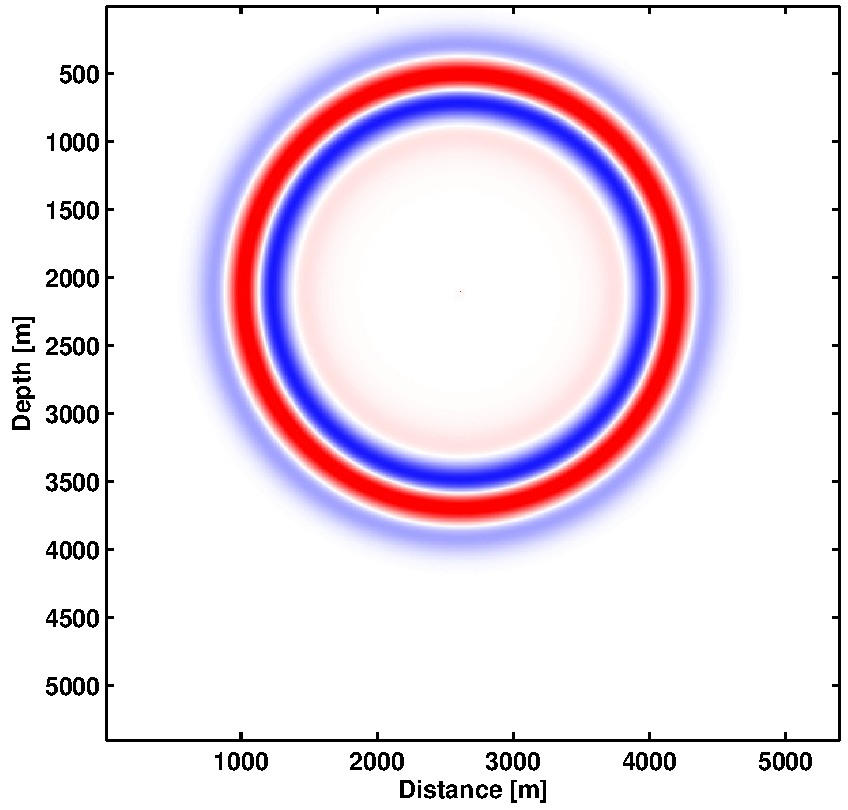
\epsfig{file=figures/homogenous_grid_n_16_5.pdf, width=6 cm}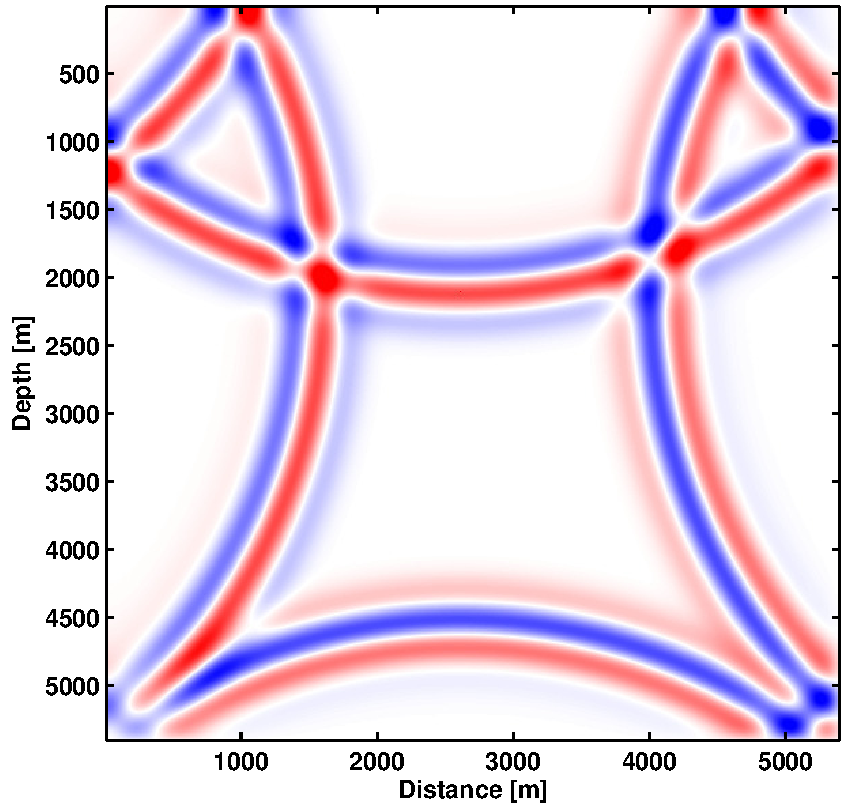
\epsfig{file=figures/homogenous_grid_n_16_10.pdf, width=6 cm}
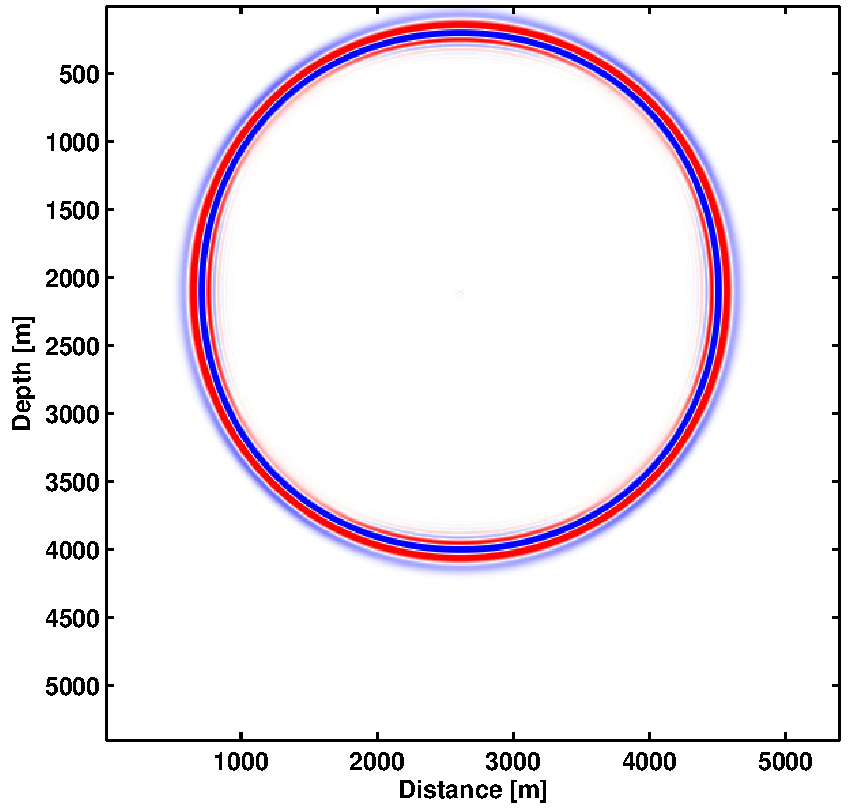
\epsfig{file=figures/homogenous_grid_n_4_5.pdf, width=6 cm}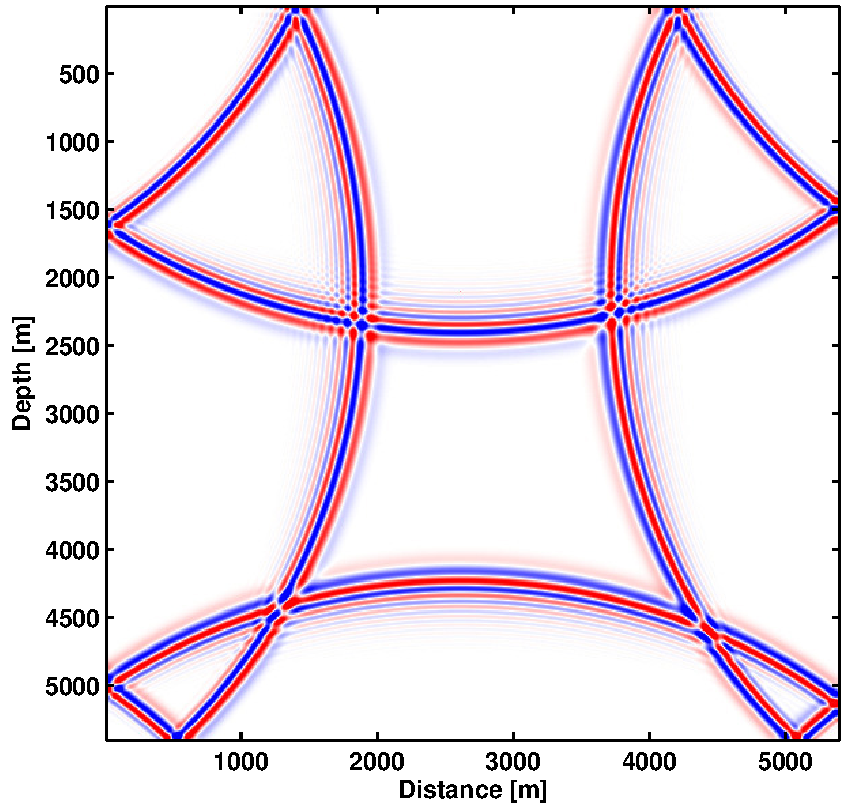
\epsfig{file=figures/homogenous_grid_n_4_10.pdf, width=6 cm}
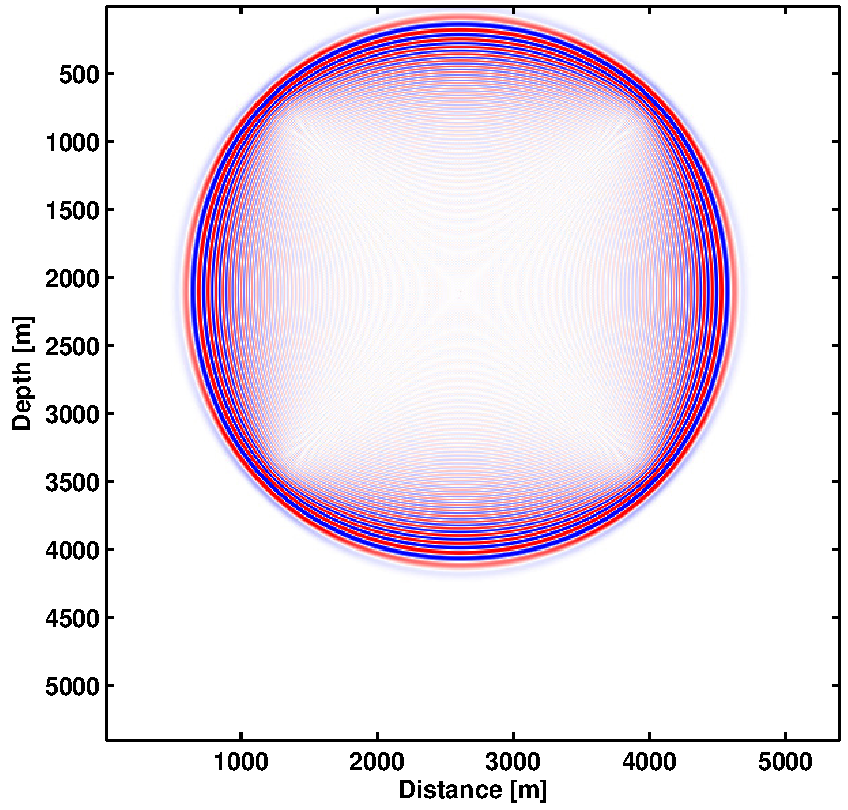
\epsfig{file=figures/homogenous_grid_n_2_5.pdf, width=6 cm}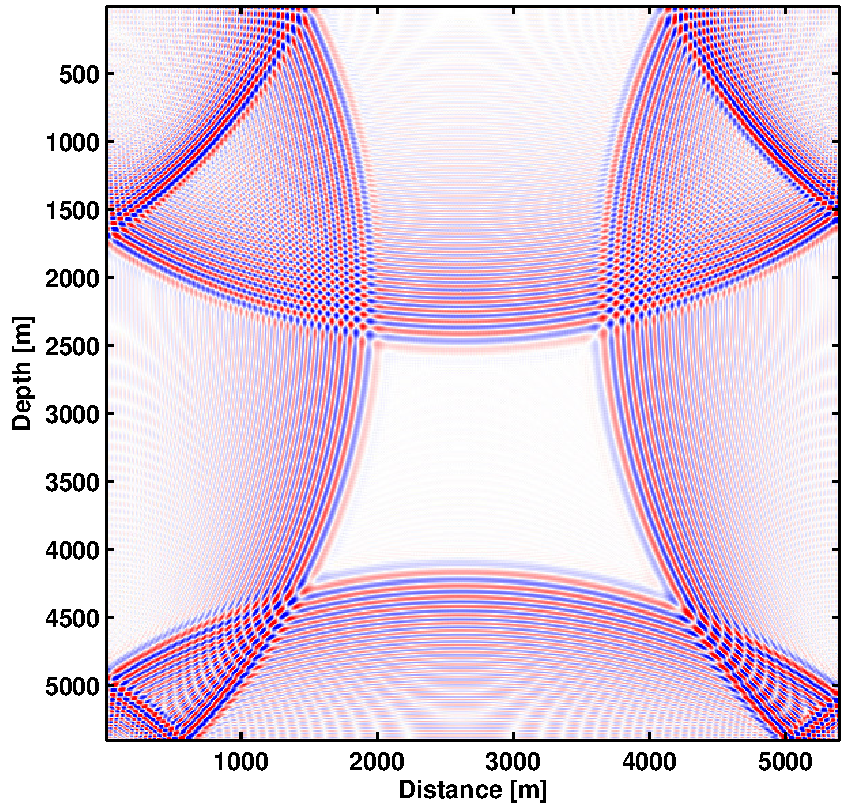
\epsfig{file=figures/homogenous_grid_n_2_10.pdf, width=6 cm}
\caption{\label{grid_disp_pics} The influence of grid dispersion in FD modeling: Spatial sampling of the wavefield using n=16 (top), n=4 (center) and n=2 gridpoints (bottom) per minimum wavelength $\rm{\lambda_{min}}$.}
\end{center}
\end{figure}
\clearpage
\subsection{The Courant Instability}\label{courant}
Beside the spatial, the temporal discretization has to satisfy a sampling criterion to ensure the stability of the FD code. If a 
wave is propagating on a discrete grid, then the timestep $dt$ has to be less than the time for the wave to travel between two adjacent grid 
points with grid spacing dh. For an elastic 2D grid this means mathematically:
\EQ{courant:1}{\rm{dt \le \frac{dh}{h \sqrt{2} V_{max}},}}
where $\rm{V_{max}}$ is the maximum velocity in the model. The factor h depends on the order of the FD operator and can easily calculated by summing over the weighting coefficients $\beta_i$
\EQ{courant:1:1}{{\rm{h} = \sum_i \beta_i.}}
In table \ref{courant.1} h is listed for different FD operator lengths and types (Taylor and Holberg operators). Criterion \ER{courant:1} 
is called {\bf{Courant-Friedrichs-Lewy criterion}} (\cite{courant:28}, \cite{courant:67}). \FIG{courant_pics} shows the evolution of the pressure field when the Courant criterion is violated. After a few time steps the amplitudes are growing to infinity and the calculation becomes unstable.
\begin{table}[hbt]
\begin{center}
\begin{tabular}{ccc}\hline \hline
FDORDER & h (Taylor)      & h (Holberg) \\ \hline 
2nd   &   1.0             &  1.0        \\
4th   &   7/6             &  1.184614   \\
6th   &   149/120         &  1.283482   \\
8th   &   2161/1680       &  1.345927   \\
10th  &   53089/40320     &  1.387660   \\
12th  &   1187803/887040  &  1.417065   \\   
\hline \hline
\end{tabular}
\caption{\label{courant.1} The factor h in the Courant criterion for different orders (2nd-12th) and types (Taylor and Holberg) of FD operators.}
\end{center}
\end{table} 
\clearpage
\begin{figure}[ht]
\begin{center}
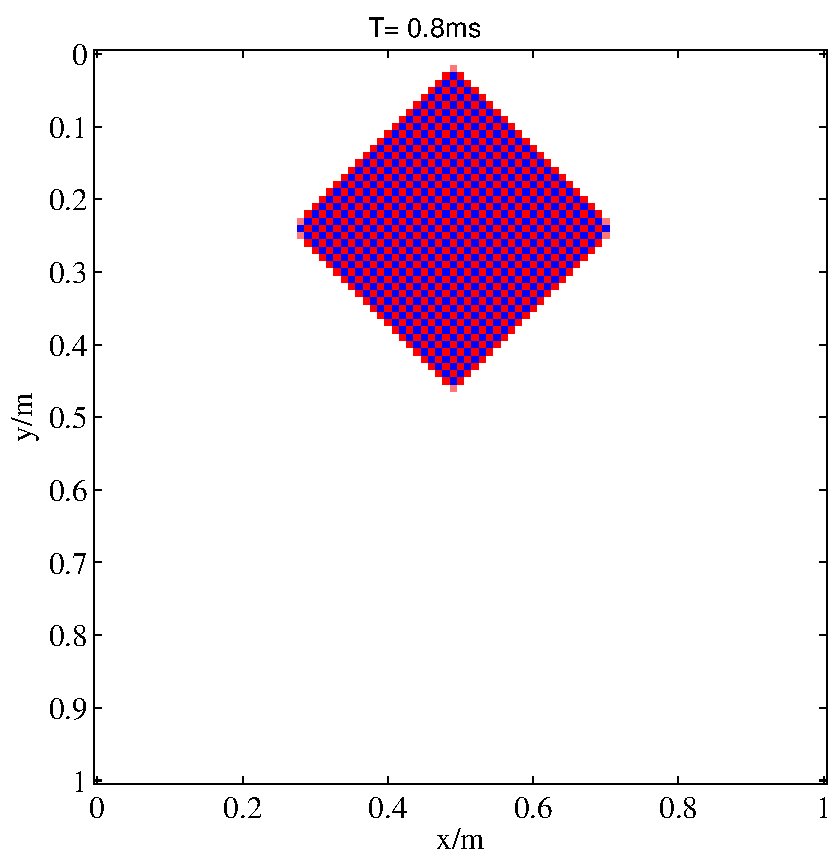
\epsfig{file=figures/courandt_1.pdf, width=7 cm}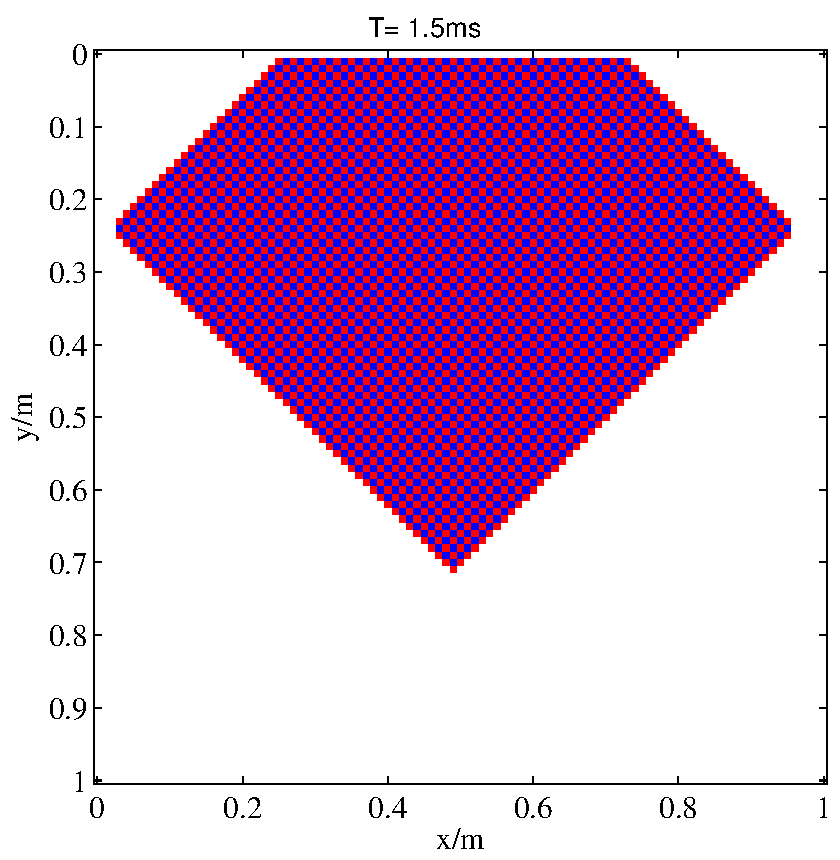
\epsfig{file=figures/courandt_2.pdf, width=7 cm}
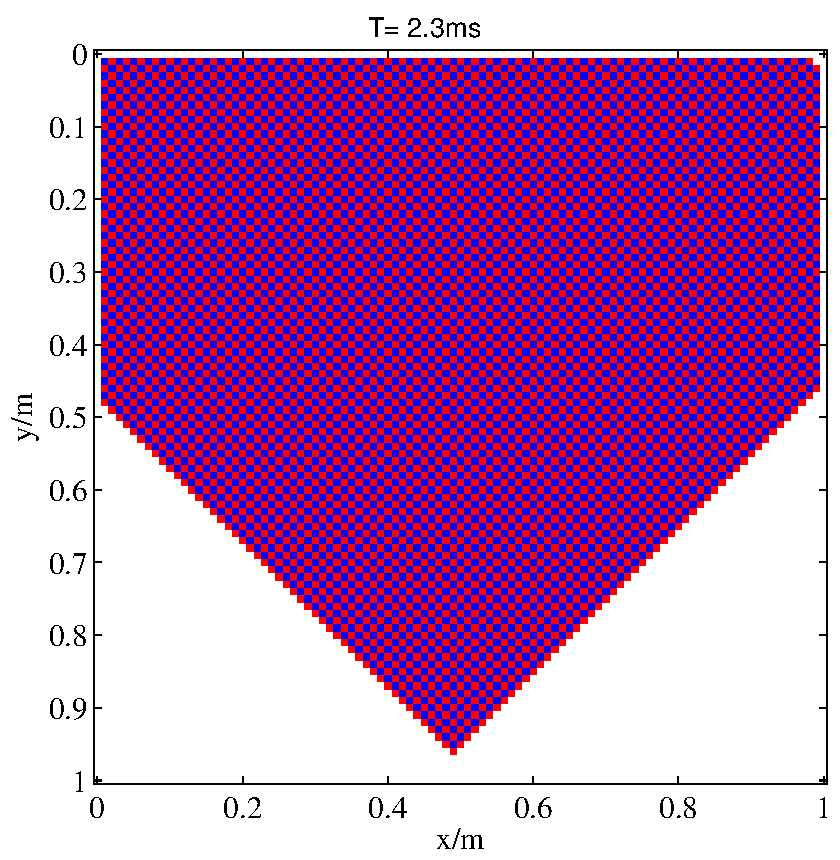
\epsfig{file=figures/courandt_3.pdf, width=7 cm}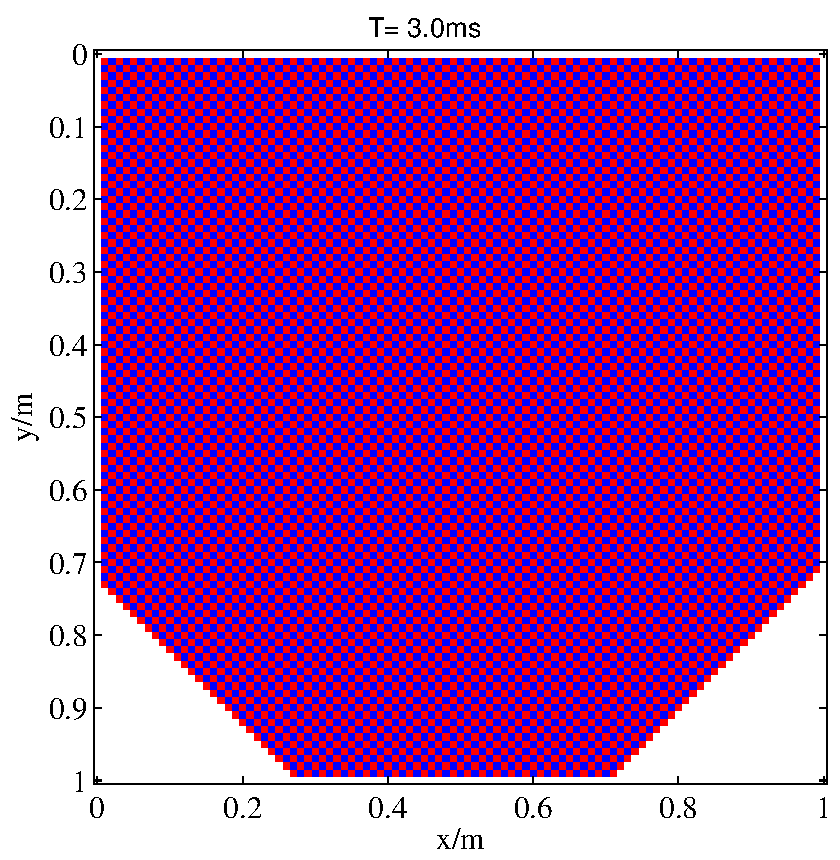
\epsfig{file=figures/courandt_4.pdf, width=7 cm}
\caption{\label{courant_pics} Temporal evolution of the Courant instability. In the colored areas the wave amplitudes are extremly large.}
\end{center}
\end{figure}
\clearpage

\section{Installation}
\label{installation}
In sofi2D package you will find different subdirectories:

\textbf{bin}\\
This directory contains all executable programs, generally sofi2D and snapmerge. These executables are generated using the command \texttt{make $<$program$>$} (see below).

\textbf{doc}\\
This directory contains documentation on the software (this users guide).

\textbf{genmod}\\
Contains the model and benchmark files for sofi2D.

\textbf{mfiles}\\
Here some Matlab routines (m-files) are stored. These Matlab programs can be used to find optimal relaxation frequencies to approximate a constant Q (qapprox.m) or to plot Q as a function of frequency for
certain relaxation frequencies and value of tau (qplot.m). For further details on the theory behind these algorithms we refer to the Phd thesis of T. Bohlen \cite{bohlen:98} and to the paper in which the so-called tau-method is described \cite{blanch:95}. The parameter tau is used in this software to define the level of attenuation.

\textbf{overnightbuilt}\\
This directory only appears in the overnightbuilt version of SOFI2D.
This directory contains a complete bechmarking suite designed to test whether your installed release of SOFI2D works as intended. During the test run, several model scenarios will be simulated and ,afterwards, the created seismogram and snapshot files will be compared with reference values created by the SOFI2D developer team. This benchmarking test can be used as an overnight built check while developing the code, i.e. after modifications to the code, the test evaluates if standard modeling scenarios still result in the same simulation output. For further information we refer to the separate documentation \texttt{sofi2D\_overnight\_documentation} located in the folder \textbf{doc}.

\textbf{par}\\
Parameter files for sofi2D modeling.

\textbf{src}\\
This directory contains the complete source codes.  The following programs are available and my be compiled using \texttt{make $<$program$>$}.


\begin{table}[hbt]
\begin{tabular}{ll}
program & purpose \\ \hline
\texttt{snapmerge} & program to merge snapshot files \\
\texttt{sofi2D} & Viscoelastic/elastic code,  2nd-12th order spatial FD operators, SSG \\
\texttt{sofi2D\_bench} & Viscoelastic/elastic code,  2nd-12th order spatial FD operators, SSG, \\
& only used for Overnight built testing suite \\
\end{tabular}
\caption{Names of excecutables located in the folder \textbf{bin} and purpose}
\label{tab_programs}
\end{table}

\section{Example problem: Homogenous block model}
\label{simple test}
\subsection{Preliminary Considerations}
To illustrate the usage of sofi2D we use a homogenous block model adapted from \cite{kang:04} with the dimensions 5400.0 x 5400.0 m. The material parameters of the block are:  P-wave velocity $v_p=3500.0\; \frac{\mathrm{m}}{\mathrm{s}}$, S-wave velocity $v_s=2000.0\; \frac{\mathrm{m}}{\mathrm{s}}$ and density $\rho=2000.0\; \frac{\mathrm{kg}}{\mathrm{m}^3}$. An explosive source is located inside the model at point  $x_s=2592.0\;$m and $y_s=2106.0\;$ km (y denotes the vertical direction). The source function is a Ricker wavelet (see Chapter \ref{sources}) with a center frequency $f_c$ of 5 Hz. To calculate the dimensions of the grid the spatial grid spacing is estimated using the grid dispersion criterion. For an 8th order Holberg FD operator using $v_{s,min}=2000\;$m/s, $f_{max}=2 \cdot f_c=10\;$ Hz and $\rm n=3.69$ we get:

\EQ{prob1:1}{\rm{dh} \le \frac{V_{s,min}}{n\; f_{max}} = 54.2\;\mathrm{m}.}

The whole model grid has the dimensions 100 x 100 gridpoints. To avoid a violation of the Courant criterion the time step size DT is calculated according to using $v_{p-max}=3500\; m/s$, $\rm h=1.345$ and $\rm{dh=54.0\; m}$:

\EQ{prob1:2}{\rm{DT} \le \frac{\rm{dh}}{h \sqrt{2} v_{p-max}} = 6.62\times 10^{-3} s \approx 6.6\; \mathrm{ms}.}

The modeling covers a time span of 5.0 s, so about NT=649 time steps are needed. A line of 100 Geophones is placed between $x_{start}=54.0\;$ m and $x_{end}=5400.0\;$ m and a constant depth of $y=2106.0\;$m. Please note, that due to the small size of the model, more than half of the grid is covered by the absorbing boundary (see Chapter \ref{abs}). 

\subsection{Definition of the Wave Modeling Parameters}
\label{modelgeom}
The geometry of the FD grid and all parameters for the wave field simulation have to be defined in a parameter file (which we name in this case {\texttt{sofi2D/par/in\_and\_out/sofi2D.json}}). In the following we will first list the full input file and later explain every input parameter section in detail:
\input{sofi2D.json}
All lines in the parameter file are formated according to the JSON standard (\url{http://www.json.org}) and organized as follows: 

\begin{verbatim}
"VARNAME" = "Parameter value",
\end{verbatim}

a comment line can look like this

\begin{verbatim}
"Comment" = "This is a useful comment",
"3D Grid information" = "comment",
\end{verbatim}

where VARNAME denotes the name of the global variable in which the value is saved in all functions of the program. The possible values are described in comments, feel free to add own comments. Basically all non JSON conform line will be ignored. The order of parameters can be arbitrary organized. The built-in JSON parser will search for the need parameters and displays found values. If critical parameters are missing the code will stop and an error message will appear. The meaning of the different parameters is described in the following.

\begin{figure}
\begin{center}
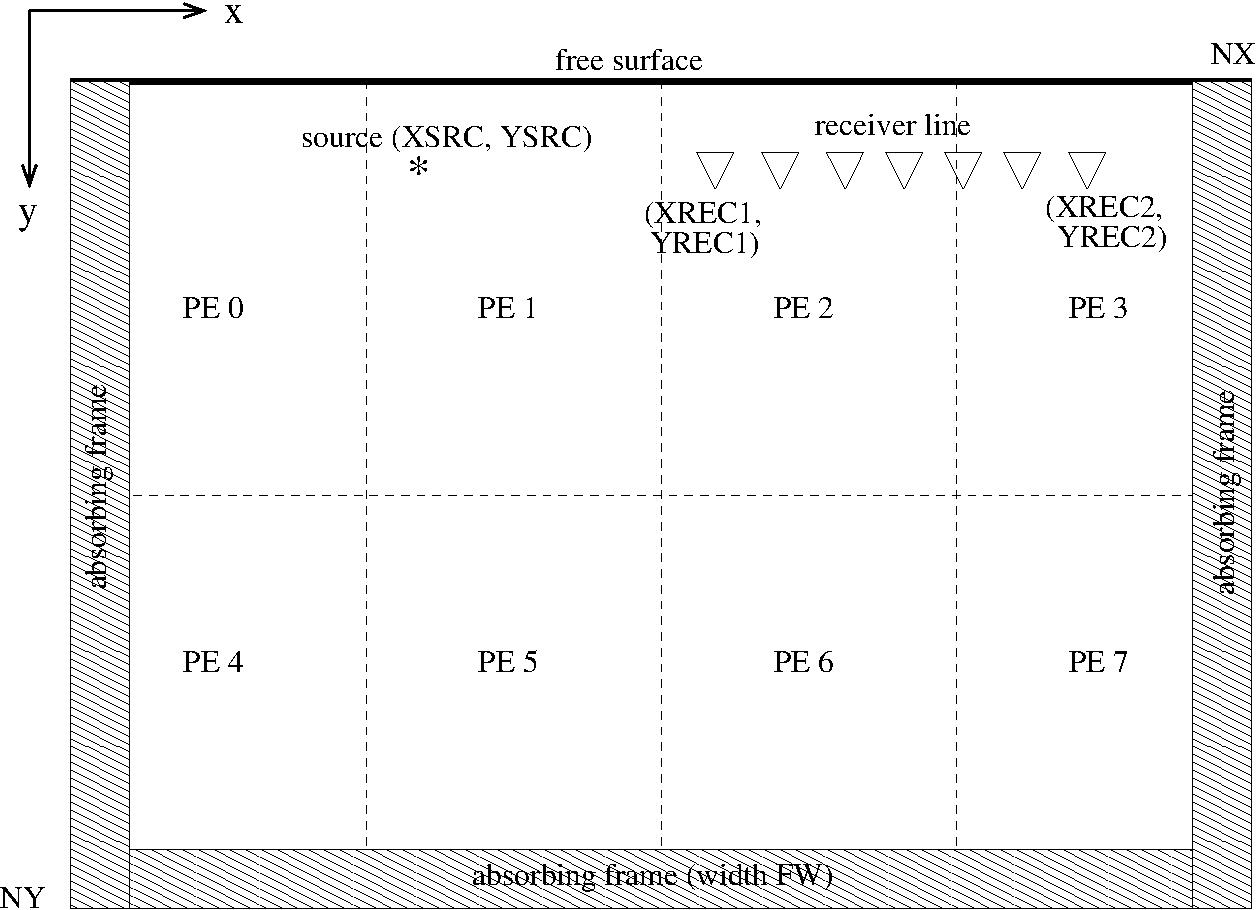
\includegraphics[width=15cm,angle=0]{figures/grid.pdf}
\end{center}
\caption{Geometry of the numerical FD grid using 4 processors in x direction (NPROCX=4) and 2 processors in y-direction (NPROCY=2). Each processing element (PE) is updating the wavefield in his domain.
At the top of the numerical mesh the PEs apply a free surface boundary condition if FREE\_SURF=1, otherwise an absorbing boundary condition is applied. The width of the absorbing frame is FW meters. The size of the total grid is NX grid points in x-direction and NY gridpoints in y-direction. The size of each subgrid thus is NX/NPROCX x NY/NPROCY gridpoints. The source is located at (XSRC,YSRC). The first receiver is at (XREC1,YREC1) and the last receiver at (XREC2,YREC2). The origin of the cartesian coordinate system is at the top left corner of the grid. }
\label{fig_grid}
\end{figure}
\newpage
\subsubsection{Domain decomposition}

\begin{verbatim}
"Domain Decomposition" : "comment",
			"NPROCX" : "2",
			"NPROCY" : "2",
\end{verbatim}

with

NPROCX : number of processors in x-direction \newline
NPROCY : number of processors in y-direction

Parallelization is based on domain decomposition (see Figure \ref{fig_grid}), i.e each processing element (PE) updates the wavefield within his portion of the grid. The model is  decomposed by the program into subgrids. After decomposition each processing elements (PE) saves only his sub-volume of the grid. NPROCX and NPROCY specify the number of processors in x- and y-direction, respectively (Figure  \ref{fig_grid}). The total number of processors thus is NP=NPROCX*NPROCY. This values must be specified when starting the program with the mpirun command: \texttt{mpirun -np $<$NP$>$ ../bin/sofi2D $<$ sofi2D.json}. If the total number of processors in sofi2D.json and the command line differ the program will terminate immediately with a corresponding error message. Obviously, the total number of PEs (NPROCX*NPROCY) used to decompose the model should be less equal than the total number of CPUs which are available on your parallel machine. If you use LAM and decompose your model in more
domains than CPUs are available two or more  domains will be updated on the same CPU (the program will not terminate and will produce the correct results). However, this is only efficient if multi-core processors are installed on your machine. In order to reduce the amount of data transferred between PEs one should try to realize more or less cubic subgrids. In our example, we use 2 PEs in each direction: NPROCX=NPROCY=2. The total number of PEs used by the program is NPROC=NPROCX*NPROCY=4. 

\subsubsection{Order of the FD operator}
\begin{verbatim}
"FD order" : "comment",
			"FDORDER" : "2",
			"FDORDER_TIME" : "2",
			"MAXRELERROR" : "1",
\end{verbatim}

with \\ 
FDORDER : Order of ssg FD coefficients (values: 2, 4, ..., 12)\newline
FDORDER TIME : Order of temporal FD coefficients (values: 2 and 4)\newline
MAXRELERROR : Maximum relative group velocity error E and minimum number of grid points per shortest wavelength, values:\newline
	0 = Taylor coefficients\newline
	1 = Holberg coeff.: E = 0.1 \% \newline
  	2 =                 E = 0.5 \% \newline
	3 =                 E = 1.0 \% \newline
	4 =                 E = 3.0 \% \newline

The order of the used FD operator is defined by the option FDORDER. In the current FD software, 2nd, 4th, 6th, 8th, 10th and 12th order operators are implemented. The variable FDORDER\_TIME represents the used temporal FD order. FDORDER\_TIME=2 correspondents to the classical leapfrog scheme and FDORDER\_TIME=4 to a fourth order accurate scheme. By the option max\_relative\_error the user can switch between Taylor (0) and Holberg (1) FD coefficients or define a maximum of tolerated group velocity error in \%. The chosen FD operator and FD coefficients have an influence on the numerical stability and grid dispersion (see next chapter).

\subsubsection{Discretization}

\begin{verbatim}
"2-D Grid" : "comment",
			"NX" : "100",
			"NY" : "100",
			"DH" : "54.0",
\end{verbatim}

These lines specify the size of the total grid (Figure  \ref{fig_grid}). NX and NY give the number of grid points in the x- and y-direction, respectively, and DH specifies the grid size. An equidistant grid is used in the FD software. DH thus is the distance between gridpoints in both spatial directions. The size of the total grid in meters in x-direction is NX*DH and in y-direction NY*DH.
\textbf{Note that the y-direction always corresponds to the vertical direction, i.e. to depth!}. NX/NPROCX and NY/NPROCY must be integer values.

To avoid numerical dispersion the wavefield must be discretized with a certain number of gridpoints per wavelength. The number of gridpoints per wavelength required depends on the order of the spatial
FD operators used in the simulation. In the current FD software only second and 4th order operators are used (Table \ref{tab_programs}). The criterion to avoid numerical dispersion reads:
\begin{equation}
DH\le\frac{Vs_{min}}{2 f_c N} \label{eq_dispersion}
\end{equation}
where $\frac{Vs_{min}}{2 f_c}$ is the smallest wavelength propagating through the model. $vs_{min}$ denotes the minimum shear wave velocity in the model, and $f_c=1/TS$ is the center frequency of the source wavelet. The program assumes that the maximum frequency of the source signal is approximately two times the center frequency. To avoid numerical dispersion of body waves 8 grid points per minimum wavelength ($N=8$) are necessary for a 4th order algorithm and  $N=12$ grid points for a second order algorithm (Table \ref{tab_programs}). Modeling Rayleigh waves without applying explicit boundary conditions may require finer sampling \cite{bohlen:06}. The criterion \ref{eq_dispersion} is checked by the FD software. See the sofi2D output file (default: sofi2D.jout), section ``--- CHECK FOR GRID DISPERSION ---`` for further information or warnings. Please note, that the FD-code will NOT terminate due to grid dispersion.

\subsubsection{Time stepping}
\begin{verbatim}
"Time Stepping" : "comment",
			"TIME" : "5.0",
			"DT" : "8.0e-3",
\end{verbatim}
The propagation time of seismic waves in the entire model is TIME. The time stepping interval (DT) has to fullfill the stability criterion (equation 13 in Bohlen \shortcite{bohlen:02}). The stability criteria for the different programs listed in Table \ref{tab_programs} are: 

4th order standard staggered grid (SSG):
\begin{equation}
DT \le \frac{6 DH}{7\sqrt{D} v_p^{max}}
\label{eq_stab_ssg4}
\end{equation}

second order standard staggered grid (SSG):
\begin{equation}
\rm{DT} \le \frac{DH}{\sqrt{D} v_p^{max}}
\label{eq_stab_ssg2}
\end{equation}

where $v_p^{max}$ is the maximum P-wave velocity at maximum frequency traveling within  the model. D is the dimension of the model, i.e. $D=2$ for a 2-D simulation (sofi2D) and $D=3$ for a 3-D simulation (sofi2D). The stability criteria \ref{eq_stab_ssg4} and \ref{eq_stab_ssg2} are checked by the FD software for the entire model. If the criterion is violated, the FD program will terminate with a corresponding error message. The maximum value for DT at the stability  limit is output. So you may simply try a large number, start the program and see what the program suggests for the time step interval.

\subsubsection{Sources}
\label{sources}
\begin{verbatim}
"Source" : "comment",

			"SOURCE_SHAPE" : "1",
			"SOURCE_TYPE" : "1",
			"PLANE_WAVE_DEPTH" : "0.0",
			"PLANE_WAVE_ANGLE" : "0.0",
			"TS" : "0.02",
	
			"SIGNAL_FILE" : "signal_mseis.tz",
			"SRCREC" : "1",
			"SOURCE_FILE" : "./sources/source.dat", 
			"RUN_MULTIPLE_SHOTS" : "0",
\end{verbatim}

with

SOURCE\_SHAPE : Shape of source-signal (ricker=1,fumue=2, from SOURCE\_FILE=3, sinus$^3$=4),  \newline
SOURCE\_TYPE : Point source (explosive=1;force in x=2;force in y=3),\newline
PLANE\_WAVE\_DEPTH : Depth of plane wave excitation (no=0) (in meter)\newline
PLANE\_WAVE\_ANGLE : Dip of plane wave from vertical (in degrees)\newline
TS : Duration of source-signal (in seconds)\newline
SIGNAL\_FILE : External signal file name \newline
SRCREC : Read source positions from external SOURCE\_FILE (yes=1)\newline
RUN\_MULTIPLE\_SHOTS : Multiple shots modeled simultaneously (0) or individually (1)\newline

Three built-in wavelets of the seismic source are available. The corresponding time functions are defined in src/wavelet.c. You may modify the time functions in this file and recompile to include your own analytical wavelet or to modify the shape of the built-in wavelets.

Ricker wavelet:
\begin{equation}
r(\tau)=\left(1-2\tau^2\right)\exp(- \tau^2) \quad \mbox{with} \quad \tau=\frac{\pi(t-1.5/f_c-t_d)}{1.0/f_c} 
\label{eq_ricker}
\end{equation}


Fuchs-M\"uller wavelet:
\begin{equation}
f_m(t)=\sin(2\pi(t-t_d)f_c)-0.5\sin(4\pi(t-t_d)f_c) \quad \mbox{if} \quad t\in[t_d,t_d+1/fc] \quad \mbox{else} \quad fm(t)=0
\label{eq_fm}
\end{equation}

$sin^3$ wavelet:
\begin{equation}
s3(t)=0.75 \pi f_c \sin(\pi(t+t_d)f_c)^3\quad \mbox{if} \quad t \in[t_d,t_d+1/fc] \quad \mbox{else} \quad s3(t)=0
\label{eq_s3}
\end{equation}

In these equations t denotes time and $f_c=1/TS$ is the center frequency. $t_d$ is a time delay which can be defined for each source position in SOURCE\_FILE. Variable time delays for different sources locations allow the simulation of passive acoustic emission. Note that the symmetric (zero phase) Ricker signal is always delayed by $1.5/f_c$, which means that after one and a half period the maximum amplitude is excited at the source location. These three source wavelets and the corresponding amplitude spectra for a center frequency of $f_c=50$ Hz and a delay of $t_d=0$ are plotted in Figure \ref{fig_source_wavelets}. Note the delay of the Ricker signal described above. The  Fuchs-M\"uller wavelet has a slightly higher center frequency and covers a broader frequency range.

\begin{figure}
\begin{center}
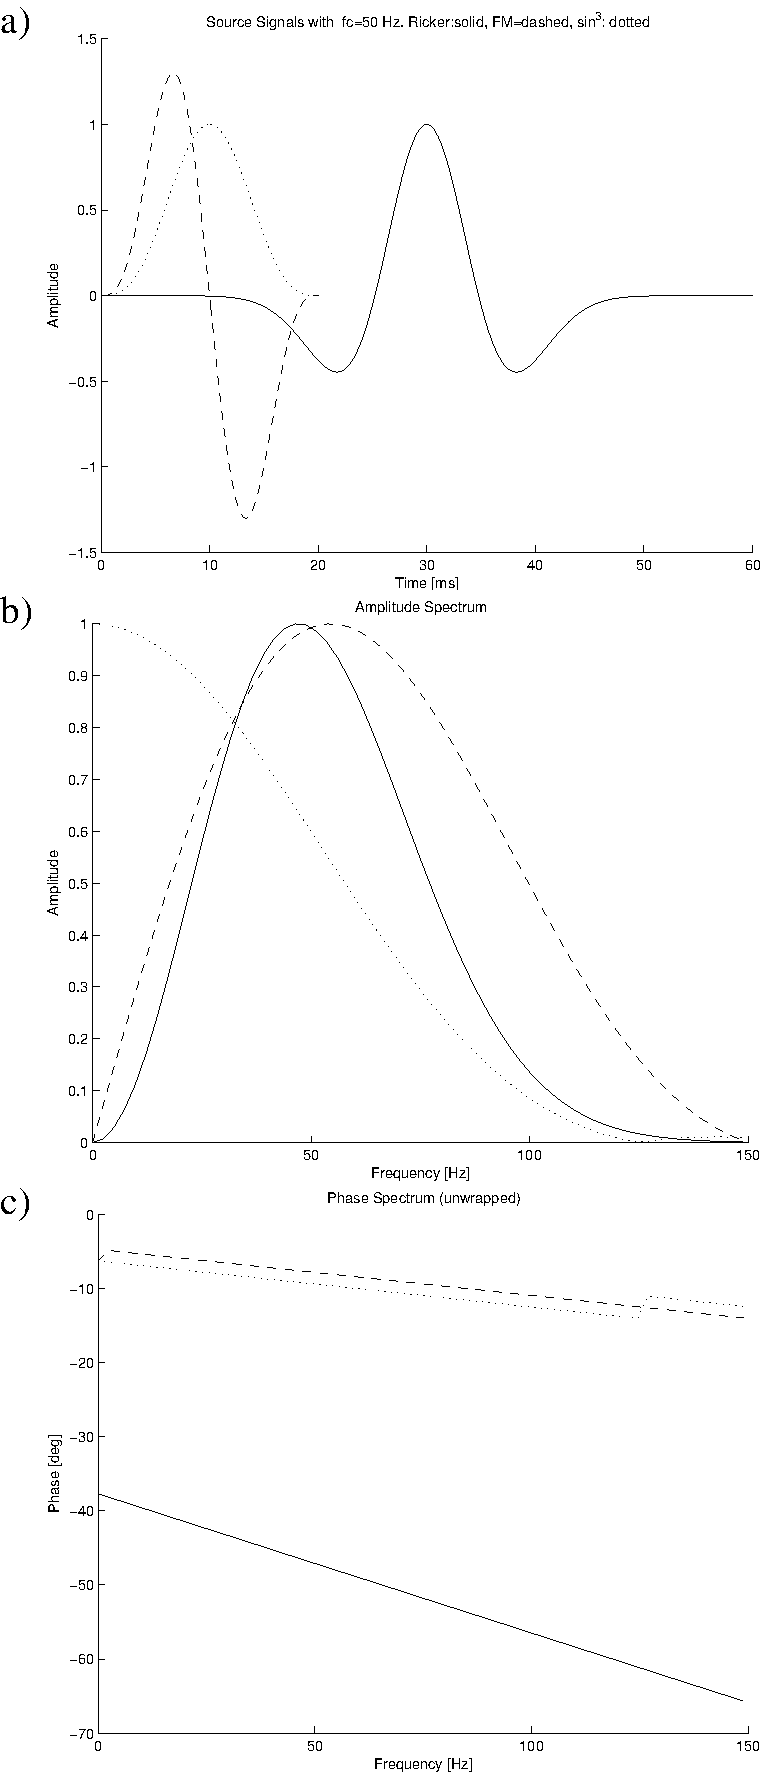
\includegraphics[width=8cm,angle=0]{figures/signals.pdf}
\end{center}
\caption{Plot of built-in source wavelets (equations \ref{eq_ricker}, \ref{eq_fm}, \ref{eq_s3}) for a center frequency of $f_c=50$ Hz 
($TS=1/f_c=0.02$s): Ricker signal (solid), Fuchs-M\"uller signal (dashed), $sin^3$-signal (dotted). a) Time function, b) amplitude
spectrum, c) phase spectrum.}
\label{fig_source_wavelets}
\end{figure}

You may also use your own digitized time function as the source wavelet (for instance the signal of the first arrival recorded by a geophone at near offsets). Specify SOURCE\_SHAPE=3 and save the samples of your source wavelet in ASCII-format in SIGNAL\_FILE. SIGNAL\_FILE should contain one sample per line. It should thus look like:

0.0\\
0.01\\
0.03\\
...\\

The time interval between the samples must equal the time step interval (DT) of the FD simulation (see above) ! It it therefore mostly necessary to resample/interpolate a given source time function with a smaller sample rate. 

The parameter SOURCE\_TYPE specifies the type of the source. SOURCE\_TYPE=1 means an explosive source which excites P-waves only radiating with the same amplitude into all directions. SOURCE\_TYPE=2, and SOURCE\_TYPE=3 simulate point forces in x- and y-direction, respectively. With  SOURCE\_TYPE=4 a source in a user-defined direction can be chosen which is defined by the parameter SOURCE\_AZIMUTH specified in in the SOURCE\_FILE (see Figure \ref{fig_source_azimuth}). The unit is in degree from 0 to 360. A SOURCE\_AZIMUTH=0 corresponds to the case SOURCE\_TYPE=3, SOURCE\_AZIMUTH=90  corresponds to SOURCE\_TYPE=2. Please note that there is a numerical inaccuracy between SOURCE\_TYPE=2 and its analog version SOURCE\_AZIMUTH=90. These sources have specific radiation characteristics and excite both P- and S-waves. In case of an explosive source the diagonal components of the stress tensor are assigned with the source wavelet. In case of a directive force in x- or y-direction, respectively, the corresponding external body force component ($f_i$, see equation 11 of Bohlen \shortcite{bohlen:02}) is assigned with the source wavelet amplitudes. Please not, that due to the 2-D FD scheme, a point force is physically described as a line source. The excited wavefield is therefore not directly comparable to a 3-D wave propagation. For a 1-D media, there is a 2-D to 3-D conversion of both body and surface waves.

\begin{figure}
\begin{center}
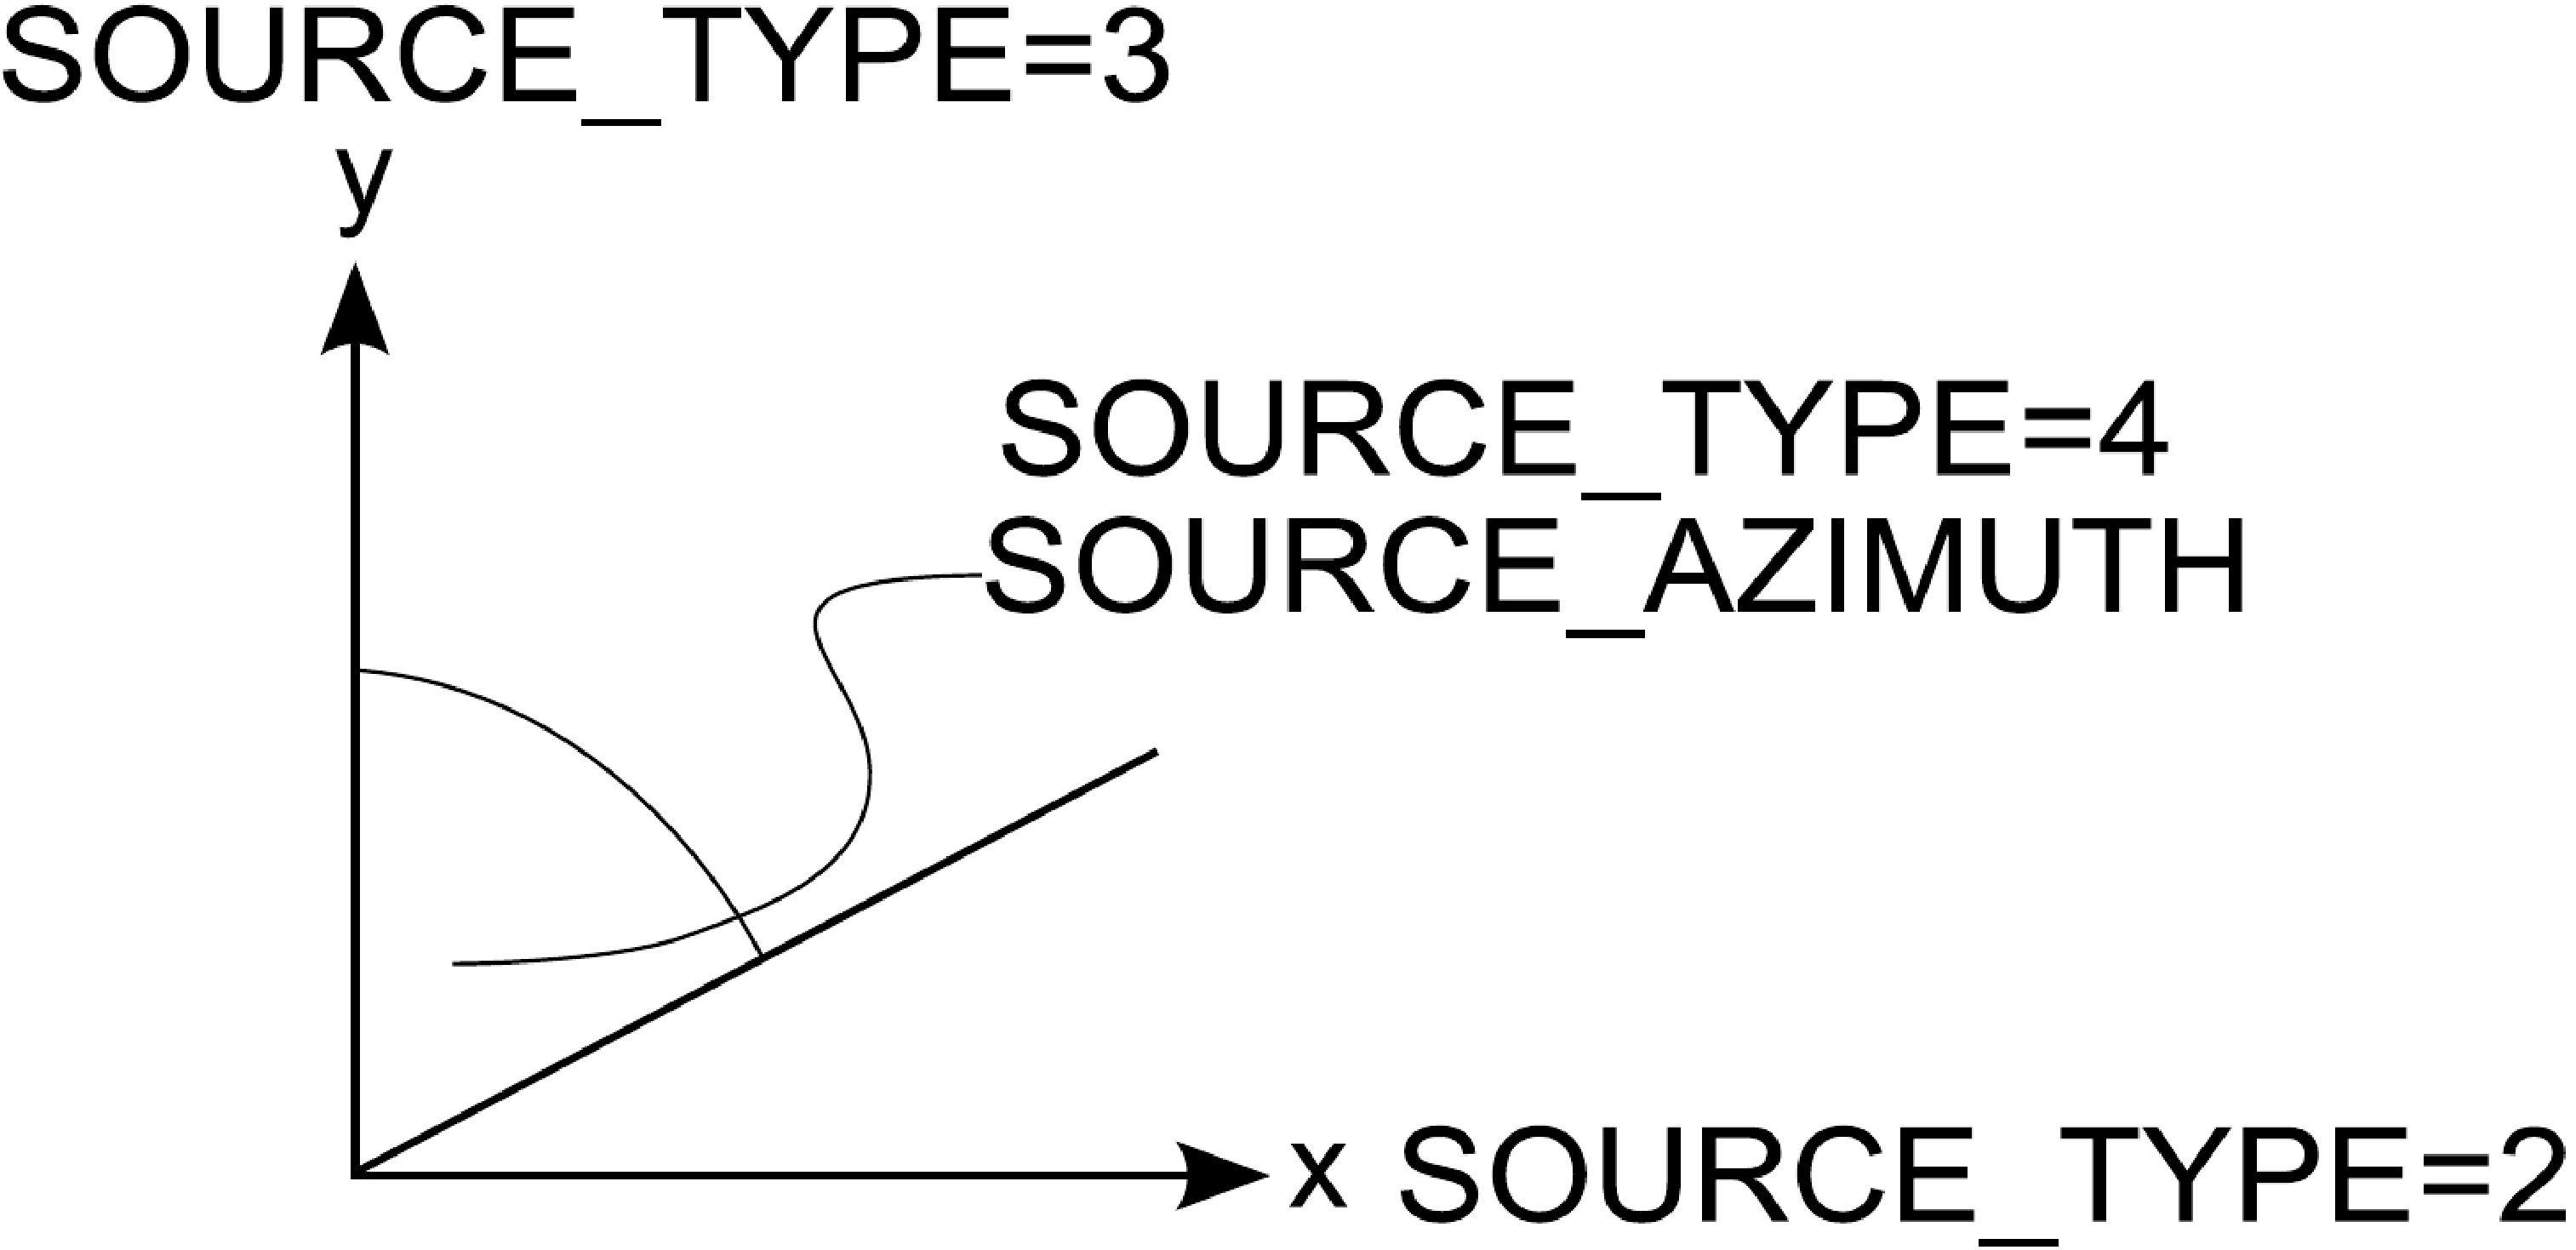
\includegraphics[width=9cm,angle=0]{figures/source_azimuth.pdf}
\end{center}
\caption{Scheme for SOURCE\_TYPE=4. The parameter SOURCE\_AZIMUTH denotes the angle between the vertical y- and horizontal x-coordinate.}
\label{fig_source_azimuth}
\end{figure}

In some applications, e.g. transmission experiments or the simulation of teleseismic events, the generation of plane waves are required.  If you specify a PLANE\_WAVE\_DEPTH greater than zero a plain wave at a depth of PLANE\_WAVE\_DEPTH is excited. In case of PLANE\_WAVE\_DEPTH $\le$ 0 point sources are applied. In this case SRCREC should be set to 1, otherwise no sources are applied.
This only makes sense if you continue a previous simulation by reading the wavefield from a checkpoint file (CHECKPTREAD=1, see below). The plane wave is simply generated by applying the source time function (SOURCE\_SHAPE) with the source characteristic (SOURCE\_TYPE) at each grid point along a straight line (2-D modeling) or a planar plane (3-D modeling). You can also excite plane waves with a certain dip from the vertical (y-) direction. See Figure \ref{fig_plane_wave} for a description of the geometry for the generation of dipping plane waves. In case of plane waves the duration of the source signal, and hence the center frequency of the source (1/TS), is specified by TS in the parameter file. In case of point sources (PLANE\_WAVE\_DEPTH=0.0 and SRCREC=1) the center frequency is defined in SOURCE\_FILE together with the location and the time delay. In case of point sources the parameter TS is ignored.

\begin{figure}[htb]
\begin{center}
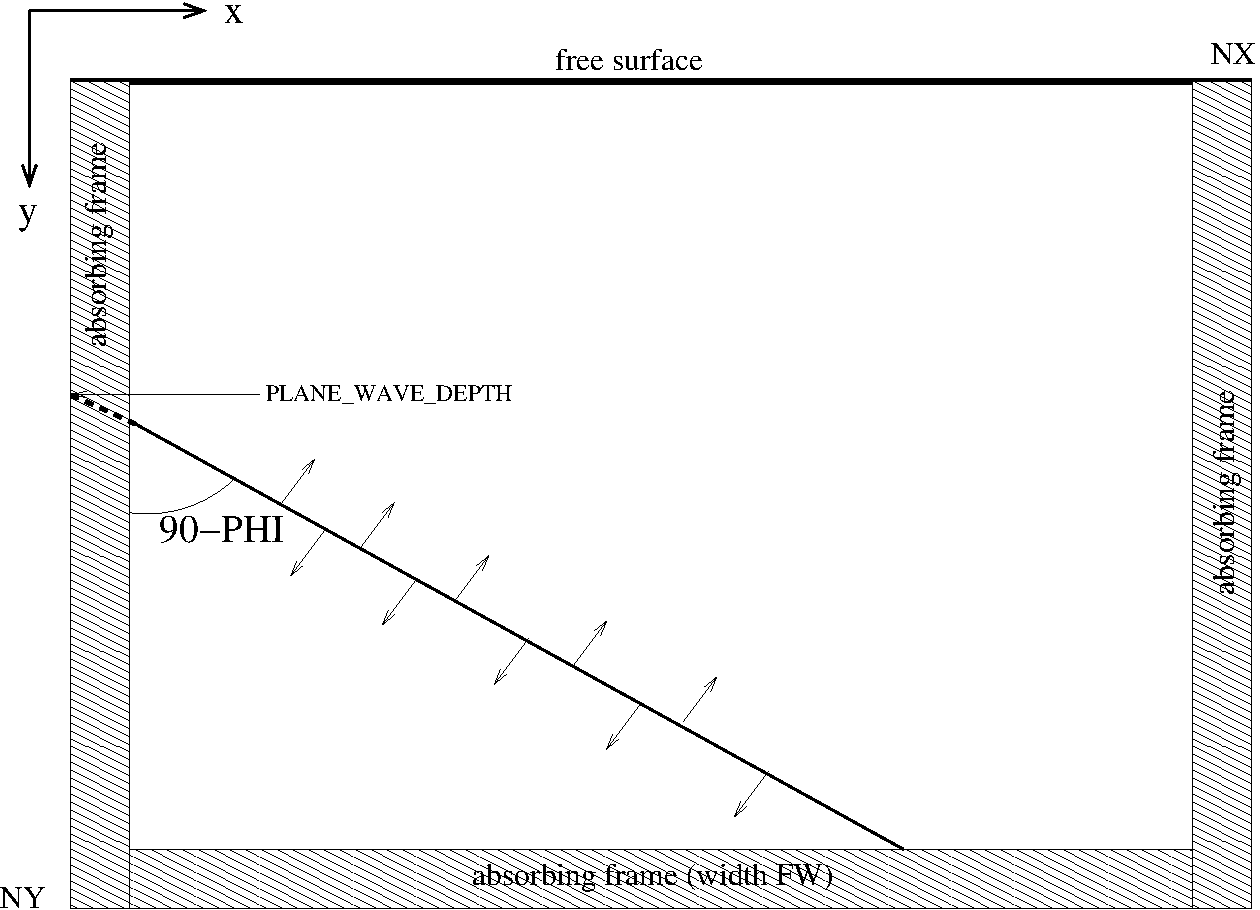
\includegraphics[width=12cm,angle=0]{figures/plane_wave.pdf}
\end{center}
\caption{Plane waves are generated by assigned source points along  straight lines (2-D simulation) or planar planes (3-D simulation) with the source wavelet. The parameter PLANE\_WAVE\_DEPTH defines the depth of this line/plane at x=0, and the parameter PLANE\_WAVE\_ANGLE specifies the incidence angle with respect to the vertical direction (PLANE\_WAVE\_ANGLE=0 corresponds to vertical incidence (directly from below)).}
\label{fig_plane_wave}
\end{figure}

For the definition of multiple point forces generate an ASCII file (SOURCE\_FILE) with the following format:
\begin{verbatim}
XSRC     YSRC     TD     FC     AMP      SOURCE_AZIMUTH     SOURCE_TYPE
\end{verbatim}

You have to define certain parameters for each source point:\newline
XSRC is the x-coordinate of a source point [in meter],\newline
YSRC is the y-coordinate (depth) of a source point [in meter],\newline
TD is the excitation time (time-delay) for the source point [in seconds],\newline
FC is the center frequency of the source signal [in Hz] and\newline
AMP is the maximum amplitude of the source signal.

Optional parameter:\newline
SOURCE\_AZIMUTH if SOURCE\_TYPE is 4, SOURCE\_AZIMUTH is the angle between the y- and x-direction,\newline
SOURCE\_TYPE if SOURCE\_TYPE is set here, the value of SOURCE\_TYPE in the input file is ignored.

The SOURCE\_FILE = \texttt{./sources/source.dat} that defines an explosive source at $x_s=2592.0\;$~m and $y_s=2106.0\;$~m (depth) with a center frequency of 5 Hz and an amplitude of 1 (no time delay) reads, for example
\begin{verbatim}
	2592.0        2106.0        0.0           5.0           1.0
\end{verbatim}

The parameter RUN\_MULTIPLE\_SHOTS defines if multiple shots are modeled simultaneously or whether each shot is modeled individually. If the parameter is set to 0, multiple sources are modeled together. If more then one source is defined in the SOURCE\_FILE each source is ignited at the same time. For RUN\_MULTIPLE\_SHOTS = 1 every source specified in the SOURCE\_FILE is modeled individually. The SEIS\_FILE name receives the addition of the number of the shot, e.g. \texttt{test\_vx.su.shot1.0}.

\subsubsection{Generation of models}
\label{gen_of_mod}
\begin{verbatim}
"Model" : "comment",
			"READMOD" : "0",
			"MFILE" : "model/test",
			"WRITE_MODELFILES" : "0",
\end{verbatim}

with

READMOD : read model parameters from MFILE (yes=1)\newline
MFILE : String for the model file names, used to read from file and/or to write model for validation \newline
WRITE\_MODELFILES : switch to decide whether all models RHO, U, Pi (and Taup, Taus) models (WRITE\_MODELFILES=1) or only the density model (WRITE\_MODELFILES=2) are written to file. In case of WRITE\_MODELFILES=0, no model file is written to file. \newline

If READMOD=1, the P-wave, S-wave, density model grid (if L=0, see chapter \ref{Q-approximation}) and additionally the attenuation grids (if L=1) are read from external binary files. MFILE defines the basic file name that is expanded by the following extensions: P-wave model: ''.vp'', S-wave model: ''.vs'', density model: ''.rho'', P-wave attenuation model: ''.qp'', S-wave attenuation model: ''.qs''.  In the example above, the model files thus are: ''model/test.vp'' (P-wave velocity model), ''model/test.vs'' (S-wave velocity model), ''model/test.rho'' (density model), ''model/test.qp'' (P-wave attenuation model), ''model/test.qs'' (S-wave attenuation model). 

In these files, each material parameter value must be saved as 32 bit (4 byte) native float. Velocities must be in meter/second, density values in $kg/m^3$. The fast dimension is the y direction. See src/readmod.c. The number of samples for the entire model in the x-direction is NX and the number of values in the y-direction is always NY. The file size of each model file thus must be NX*NY*4 bytes. You may check the model structure using the SU command ximage: \texttt{ximage n1=$<$NY$>$ n2=$<$NX$>$ $<$ model/test.vp}.

If READMOD=0 the model is generated ''on the fly'' by sofi2D, i.e. it is generated internally before the time loop starts (see chapter \ref{model_def_func}). We would prefer this way of generating the model grids because this way the size and the discretization intervals (DH) can be controlled by the parameter file sofi2D.json. Furthermore, it is not necessary to generate (large) files by an external program. See section \ref{model_def_func} for an example function that generates the simple block model ''on the fly''. If READMOD=0 this function is called in sofi2D.c and therefore must be specified in \texttt{src/Makefile} (at the top of \texttt{src/Makefile}, see section \ref{compexec}). If you change this file, for example to change the model structure, you need to re-compile sofi2D by changing to the src directory and \texttt{make sofi2D}.

Due to the fact that the variable MFILE is also used to write the model - expanded by the string ''SOFI2D'' to file for verification (also see the output file, section ''MODEL CREATION AND OUTPUT''), you can specify, whether only the density model is written (WRITE\_MODELFILES=0) or the U, Pi, density as well as Qp and Qs models (WRITE\_MODELFILES=1). BE AWARE that the output of additional models besides density cause extra but temporal memory allocation of the size of the local subgrid times the number of models! To give an example, the file name of the density models written for verification looks like this \texttt{model/test.SOFI2D.rho}. The actual Vp and Vs models can be easily calculated from the relationship:

\begin{equation}
U = V_s \cdot V_s \cdot Rho
Pi = V_p \cdot V_p \cdot Rho \mbox{.}
\label{eq_U_PI}
\end{equation}


\subsubsection{Q-approximation}
\label{Q-approximation}
\begin{verbatim}
"Q-approximation" : "comment",
			"L" : "0",
			"FL1" : "5.0", 
			"TAU" : "0.00001",
\end{verbatim}

with 

L : Number of relaxation mechanisms (L = 0: elastic, L $>$ 0: viscoelastic) \newline
FL : Relaxation frequencies (one for each relaxation mechanism) \newline

These three lines are omitted in the elastic version (if L=0). The frequency dependence of the (intrinsic) Quality factor $Q(\omega)$ is defined by the L relaxation frequencies (FL=$f_l=2\pi/\tau_{\sigma l}$) and one value $\tau$ (see equation 5 in Bohlen \shortcite{bohlen:02}). In the current model (see model.c) these values are assigned to all gridpoints for both P- and S-waves. Thus, intrinsic attenuation is homogeneous and equal for P- and S-waves ($Q_p(\omega)=Q_s(\omega)$). However, it is possible to simulate any spatial distribution of absorption by assigning the gridpoints with different
$\tau$-values. Note that for a single relaxation mechanism (L=1) 
$Q \approx 2/\tau$ \cite{bohlen:02}. $Q(\omega)$ for L=1, FL=$f_l=70Hz$, and TAU=$\tau=0.04$
is shown in Figure 11 of Bohlen \shortcite{bohlen:02}.
The Matlab script /mfiles/qplot.m can be used to plot $Q(\omega)$ for different values of L, $f_l$ and $\tau$. The m-file qapprox.m in the same directory finds optimal values for L, $f_l$ and $\tau$ that fit a desired function $Q(\omega)=const$ in a least-squares sense.

Please note, that due to dispersive media properties the viscoelastic velocity model is only defined for the reference frequency only. In sofi2D, this reference frequency is specified as the center source frequency. At the exact reference frequency, elastic and viscoelastic models are equivalent. As a consequence, slightly smaller and larger minimum and maximum velocity values occur in the viscoelastic model.

\subsubsection{Boundary conditions}
\label{abs}
\begin{verbatim}
"Boundary Conditions" : "comment",
			"FREE_SURF" : "1",
			"BOUNDARY" : "0",

			"FW" : "10",
			"ABS_TYPE" : "1",
			"ABS_TYPE values : CPML-Boundary=1; Damping-Boundary=2" : "comment",

			"Parameter of ABS_TYPE=1" : "comment",
			"NPOWER" : "4.0",
			"K_MAX_CPML" : "1.0",
			"VPPML" : "3500.0",
			"FPML" : "5.0",

			"Parameter of ABS_TYPE=2" : "comment",
			"DAMPING" : "8.0",

\end{verbatim}

with

FREE\_SURF : free surface at the top of the model (yes=1) \newline
BOUNDARY : apply periodic boundary condition at edges (no=0) (left and right=1) 

FW : width of absorbing frame (in grid points) (No=0.0) \newline
ABS\_TYPE: Type of the absorbing boundary \newline 

A plane stress free surface is applied at the top of the global grid if FREE\_SURF!=0. The imaging method proposed by Levander \shortcite{levander:88} is applied (see also Robertsson\shortcite{robertsson:96}). If FW $>$0.0 exponential damping \cite{cerjan:85} is applied at the left/right, front/back and bottom of the grid. IF FREE\_SURF equals zero damping is applied also at the top of the model. The width of the damping zone is FW.

In some cases it is usefull to apply periodic boundary conditions, for example when modeling seismic wave transmission through random media \cite{bohlen:02}. If BOUNDARY equals 1 no absorbing boundaries are installed at the left/right and front/back sides of the grid. Instead, wavefield information is copied from left to right and vice versa, as well as from front to back and vice versa. The effect is, for example, that a wave which leaves the model at the left side enters the model again at the right side.
 

If ABS\_TYPE is set to 1 a convolutional perfectly matched layer (CPML) boundary condition is used. The PML implementation is based on the following papers \cite{komatitsch:07} and \cite{martin:09}. A width of the absorbing frame of FW=10-20 grid points should be sufficient. 
For the optimal realization of the PML boundary condition you have to specify the dominant signal frequency FPML occurring during the wave simulation. This is usually the center source frequency FC specified in the source file. VPPML specifies the attenuation velocity in m/s within the PML. VPPML should be approximately the propagation velocity of the dominant wave near the model boundaries.

With ABS\_TYPE=2 
DAMPING gives the attenuation in percent at the edges of the numerical grid, i.e. amplitudes are multiplied by a factor of 1-DAMPING at the edges. The width of the absorbing frame should be at least 20 gridpoints \cite{cerjan:85}. A good choice for DAMPING is 8.0 per cent \cite{cerjan:85}. For larger values, reflections at the onset of the absorbing frame might occur. In order to avoid such an impedance contrast between the model domain and the absorbing boundary layer, you may as well increase FW and decrease DAMPING.


\subsubsection{Wavefield snapshots}
\begin{verbatim}
"Snapshots" : "comment",
			"SNAP" : "4",
			"TSNAP1" : "6.6e-3",
			"TSNAP2" : "4.8",
			"TSNAPINC" : "0.2",
			"IDX" : "1",
			"IDY" : "1",
			"SNAP_FORMAT" : "3",
			"SNAP_FILE" : "./snap/test",
\end{verbatim}

with

SNAP : output of snapshots (yes\textgreater 0) (no seismograms=0; particle-velocities=1; pressure field (hydrophones)=2; curl and divergence energy=3; velocities, pressure and energy=4)\\
TSNAP1 : first snapshot (in sec)\\
TSNAP2 : last snapshot (in sec)\\
TSNAPINC : increment (in sec)\\
IDX : increment x-direction (in grid points)\\
IDY : increment y-direction (in grid points)\\
SNAP\_FORMAT : data-format (ASCII(2);BINARY(3))\\
SNAP\_FILE : basic filename\\


If SNAP$>0$, wavefield information (particle velocities, pressure, or curl and divergence of particle velocities) for the entire model is saved on the hard disk (assure that enough free space is on disk!). Each PE is writing his sub-volume to disk. The filenames have the basic filename SNAP\_FILE plus an extension that indicates the PE number in the logical processor array (see Figure \ref{fig_grid}), i.e. the PE with number PEno writes his wavefield to SNAPFILE.PEno. The first snapshot is written at TSNAP1 seconds of seismic wave traveltime to the output files, the second at TSNAP1+TSNAPINC seconds etc. The last snapshots contains wavefield at TSNAP2 seconds. Note that the file sizes increase during the simulation. The snapshot files might become quite LARGE. It may therefore be necessary to reduce the amount of snapshot data by increasing IDX and IDY and/or TSNAPINC. In order to merge the separate snapshot of each PE after the comletion of the wave modeling, you can use the program snapmerge (see Chapter \ref{installation}, section \textbf{src}). The bash command line to merge the snapshot files can look like this: \texttt{../bin/snapmerge ./in\_and\_out/sofi2D.json}.


\subsubsection{Receivers}
\begin{verbatim}
"Receiver" : "comment",
			"SEISMO" : "4",
			"READREC" : "0",
			"REC_FILE" : "./receiver/receiver.dat",
			"REFRECX, REFRECY" : "0.0 , 0.0",
			"XREC1,YREC1" : "54.0 , 2106.0",
			"XREC2,YREC2" : "5400.0 , 2106.0",
			"NGEOPH" : "1",
\end{verbatim}

with

SEISMO : output of seismograms (no seismograms=0, particle-velocities=1, pressure (hydrophones)=2, curl and div=3, everything=4)\\
READREC : read receiver positions from file (yes=1)\\
REC\_FILE : external receiver file name\\
REFREC : reference point for receiver coordinate system\\
if READREC : 1 the following three lines are ignored\\
XREC1,YREC : position of first receiver (in m) \\
XREC2,YREC2 : position of last receiver (in m)\\
NGEOPH : distance between two adjacent receivers (in gridpoints)\\


If SEISMO$>$0, seismograms are saved on hard disk. If SEISMO equals 1 x-, and y-component of particle velocity will be written according to parameters specified in Chapter \ref{seismograms}.
If SEISMO==2 pressure (sum of the diagonal components of the stress tensor) recorded at the receiver locations (receivers are hydrophones!) is written. if SEISMO=3 the curl and divergence are saved. 

The curl and divergence of the particle velocities are useful to separate between P- and S-waves in the snapshots of the wavefield. Sofi2D calculates the divergence and the magnitude of the curl of the particle velocity field \cite{dougherty:88}. The motivation for this is as follows. According to Morse and Feshbach \shortcite{morse:53} the energy of P- and S-wave particle velocities is, respectively,
\begin{equation}
E_p=\left(\lambda + 2 \mu\right) (div(\vec{v}))^2 \quad \mbox{and} \quad E_s=\mu \left|rot(\vec{v})\right|^2 \quad\mbox{.}
\label{eq_E}
\end{equation}
$\lambda$ and $\mu$ are the Lam\`{e} parameters, and $\vec{v}$ is the particle velocity vector. In order to preserve the divergence and curl sign information  while showing relative compressional
and shear particle velocity amplitudes, we plot the following quantities:
\begin{equation}
\bar{E}_p=sign(div \vec{v}) E_p^{1/2} \quad \mbox{and} \quad \bar{E}_s= sign(rot\vec{v}) E_s^{1/2} \quad\mbox{,}
\label{eq_e}
\end{equation}
The magnitudes of $\bar{E}_p$ and $\bar{E}_s$ are proportional to the magnitudes of the P- and S- particle velocities, respectively. Note that interface waves like Rayleigh waves contain both a P- and S-wave component and therefore show up on both quantities of equation \ref{eq_e}.

The locations of the receivers may either be specified in a separate file REC\_FILE or in this parameter file. If READREC=1 receiver locations are read from the ASCII-file REC\_FILE. Each line contains the coordinates of one receiver, the first two number in each line indicate the horizontal x- and vertical y-coordinate of each receiver position. To give an example of a receiver file, the following 3 lines specify 3 receivers located at constant depth (2106.0 m). However, the receiver coordinates change in x-direction (starting at 540 m) and therefore lining up along the x-axis.  
\begin{verbatim}
540.0   2106.0
1080.0  2106.0
1620.0  2106.0
\end{verbatim}
These receiver coordinates in REC\_FILE are shifted by REFREC[1] and REFREC[2] into the  x- and y-direction, respectively. This allows for completely moving the receiver spread without modifying REC\_FILE. This may be useful for the simulation of moving profiles in reflection seismics.

If READREC=0 the receiver locations must be specified in the parameter file. In this case, it is assumed that the receivers are located along a straight line. The first receiver position is defined by (XREC1, YREC1), and the last receiver position by (XREC1, YREC1). The spacing between receivers is NGEOPH grid points.  A Vertical Seismic Profile (VSP) is realized when XREC1=XREC2, YREC1$<$YREC2.  

Receivers are always located on full grid indices, i.e. a receiver that is located between two grid points will be shifted by the FD program to the closest next grid point. It is not yet possible
to output seismograms for arbitrary receiver locations since this would require a certain wavefield interpolation.

\textbf{It is important to note that the actual receiver positions defined in REC\_FILE or in sofi2D.json may vary by DH/2 due to the staggered positions of the particle velocities and stress tensor components. }

In our example, we specify 100 receiver location. Due to the small size of the model, most of the specified receiver positions will be located inside this absorbing boundary (see Chapter \ref{abs}). A corresponding warning message will appear. If you choose to read the receiver location from REC\_FILE \texttt{./receiver/receiver.dat} (READREC=1), only 10 receivers locations are considered. The list of receivers specified in file \texttt{./receiver/receiver.dat} is equivalent to the parameters in the input file with only a larger distance between adjacent receivers (NGEOPH = 10.)

\subsubsection{Receiver array}
\begin{verbatim}
"Receiver array" : "comment",

			"REC_ARRAY" : "0",
			"REC_ARRAY_DEPTH" : "70.0",
			"REC_ARRAY_DIST" : "40.0", 
			"DRX" : "4",

\end{verbatim}

A horizontal 1-D array of receivers is simulated if REC\_ARRAY$>$0. This option specifies the number of receiver planes horizontal to the surface of the model (parallel to the x-axis). The first plane is located in depth REC\_ARRAY\_DEPTH meter. The second plane in REC\_ARRAY\_DEPTH + REC\_ARRAY\_DIST, the last in REC\_ARRAY\_DEPTH + (REC\_ARRAY-1) $\times$ REC\_ARRAY\_DIST. The distance between receivers within each plane is DRX gridpoints (DRX*DH meter).

\subsubsection{Seismograms}
\label{seismograms}
\begin{verbatim}
"Seismograms" : "comment",
			"NDT" : "1",
			"SEIS_FORMAT" : "1",
			"SEIS_FILE" : "./su/test",
\end{verbatim}

with

NDT : samplingrate (in timesteps!)\\
SEIS\_FORMAT : data output format (SU (native 4-byte-floats (IEEE on PC)/little endian on PC)=1; TEXTUAL (native ASCII)=2; BINARY (IEEE-4-byte-floats on PC/little endian on PC)=3)\\
SEIS\_FILE : basic filename according to output of seismograms (SEISMO), separate seismogram files are outputted and will look like \texttt{SEIS\_FILE\_vz.su} or \texttt{SEIS\_FILE\_div.bin.0}\\


If SEISMO$>$0 seismograms recorded at the receiver positions are written to the corresponding output files. The sampling rate of the seismograms is NDT*DT seconds. In case of a small time step interval and a high number of time steps, it might be useful to choose a high NDT in order to avoid a unnecessary detailed sampling of the seismograms and consequently large files of seismogram data. Possible output formats of the seismograms are SU, ASCII or BINARY. It is recommended to use SU format for saving the seismograms. The main advantage of this format is that the time step interval (NDT*DT) and the acquisition geometry (shot and receiver locations) are stored in the corresponding SU header words. Also additional header words like offset are set by sofi2D. This format thus facilitates a further visualization and processing of the synthetic seismograms.

Note, however, that SU cannot handle sampling rates smaller than 1.0e-6 seconds and the number of samples is limited to about 32.000. In such cases, you should increase the sampling rate by increasing NDT. If this is impossible (for example because the Nyquist criterion is violated) you must choose a different output format (ASCII or binary).

Each PE internally stores seismograms which are recorded in his portion of the grid. After finishing the time step loop, the seismogram parts are internally exchanged and the merged seismograms are collectively saved to file. The filenames are expanded according to basic file name SEIS\_FILE and the SEISMO option (pressure, particle velocity, curl, divergence). To give an example, PE0 writes the merged seismograms of the x-component of particle velocity to \texttt{SEIS\_FILE\_vx.su}. 

%If SU-files are output these can be merged together by using the Unix command cat. For example to merge seismograms of the vx-component of particle velocity into one single SU-file use:
%\emph{cat SEIS\_FILE\_VR.* $>$ SEIS\_FILE\_VR} 
%The shell script \path{sucat.sh} merges all seismograms at the same time.

\subsubsection{Monitoring the simulation}
\begin{verbatim}
"Monitoring the simulation" : "comment",
			"LOG" : "1",	
			"LOG_FILE" : "log/test.log",
			"OUT_TIMESTEP_INFO" : "10",
			
\end{verbatim}

with

LOG: output of logging information of node (no output=0; to stdout=1; to file LOG\_FILE=2)\\
LOG\_FILE : log-file for information about progress of program (each PE is printing log-information to LOG\_FILE.MYID)\\


sofi2D can output a lot of useful and possibly not useful information about the modeling parameters and the status of the modeling process etc. The major part of this information is output by PE 0.
If LOG=1, PE 0 writes this info to stdout, i.e. on the screen of your shell. This is generally recommended  to monitor the modeling process. You may want to save this screen info to a output file by adding \texttt{$>$ sofi2D.jout} or \texttt{|tee sofi2D.jout}. to your starting command. If LOG=1 all other processes with PE number (PEno) greater than zero will write their information to LOG\_FILE.PEno. If you specify LOG=2 also PE 0 will output his information to LOG\_FILE.0. As a consequence only little information is written directly to the screen of your shell. On supercomputers where you submit modeling jobs to a queuing system as batch jobs LOG=2 may be advantageous. In case of LOG=2, you may still watch the simulation by checking the content of LOG\_FILE.0 for example by using the Unix commands more or tail. After finishing the program the timing information is written to the ASCII file log/test.log.0.timings. This feature is useful to benchmark your local PC cluster or supercomputer. If LOG=0 no output from node 0 will be written, neither to stdout nor to an LOG file. There will be also no output of timing information to the ASCII file log/test.log.0.timings. 

Due to the fact that the output of information on the update and exchange via fprint can be both slowing down the computation for very small models and producing large output files, you can choose by OUTNTIMESTEPINFO after how many time steps such intermediate information are given.

\subsubsection{Checkpointing}
\begin{verbatim}
"Checkpoints" : "comment",
			"CHECKPTREAD" : "0",
			"CHECKPTWRITE" : "0",
			"CHECKPT_FILE" : "tmp/checkpoint_sofi2D",
\end{verbatim}

with

CHECKPTREAD : read wavefield from checkpoint file (yes=1/no=0)\\
CHECKPTWRITE : save wavefield to checkpoint file (yes=1/no=0)\\
CHECKPTFILE : checkpoint file\\


On most supercomputers with a queuing system the run time of job is limited. Sometimes the allowed run time is not sufficient to finish a FD simulation. In such a case, check-pointing can be performed: the first job saves the complete elastic wavefield (CHECKPTWRITE=1) but does not! read the wavefield from a checkpoint file (CHECKPTREAD=0). The subsequent jobs read and write the wavefield to the CHECKPTFILE, i.e. CHECKPTREAD=1 and CHECKPTWRITE=1. In this manner, one simulation can be divided on different batch jobs. The resulting seismograms may be catenated using the SU-command sucat. But be aware that the checkpointing option saves the COMPLETE wavefield information of the last time step, which can produce a huge amount of data.

\subsection{''On the fly'' definition of material parameters}
\label{model_def_func}
If you choose to create the model ``on the fly'', the distribution of the material parameters P-wave velocity $v_p$, S-wave velocity $v-s$ and density $\rho$ for the simple block model has to be defined in the function \texttt{hh\_elastic.c} that can be found in the \texttt{src} folder.

\begin{verbatim}
/* -------------------------------------------------------------
 *   Model homogeneous half space
 *   if variable "h" is decreased, a layer over half-space is gained
 *   ------------------------------------------------------------- */

#include "fd.h"

void model_elastic(float  **  rho, float **  pi, float **  u){

	/*--------------------------------------------------------------------------*/
	/* extern variables */

	extern int NX, NY, NXG, NYG,  POS[3], MYID;
	extern int WRITE_MODELFILES;
	extern float DH;
	extern char  MFILE[STRING_SIZE];	

	/* local variables */
	float muv, piv, Vp, Vs, Rhov;
	float y;
	int i, j, ii, jj;
	char modfile[STRING_SIZE];
	float ** pwavemod=NULL, ** swavemod=NULL;


	/*-----------------material property definition -------------------------*/	

	/* parameters for layer 1 */
	const float vp1=3500.0, vs1=2000.0, rho1=2000.0, h=100000.0;


	/* parameters for layer 2 */
	const float vp2=5400.0, vs2=3700.0, rho2=2500.0;


	/*-----------------------------------------------------------------------*/

	if (WRITE_MODELFILES==1) {
		pwavemod  =  matrix(0,NY+1,0,NX+1);
		swavemod  =  matrix(0,NY+1,0,NX+1);
	}

	/* loop over global grid */
	for (i=1;i<=NXG;i++){
		for (j=1;j<=NYG;j++){

			/* calculate coordinate in m */
			y=(float)j*DH;

			/* two layer case */
			if (y<=h){
				Vp=vp1; Vs=vs1; Rhov=rho1; }


			else{
				Vp=vp2; Vs=vs2; Rhov=rho2; }

			/* homogenous case */
			// 				vp=vp1; vs=vs1; rhov=rho1;

			muv=Vs*Vs*Rhov;
			piv=Vp*Vp*Rhov;

			/* only the PE which belongs to the current global gridpoint
				  is saving model parameters in his local arrays */
			if ((POS[1]==((i-1)/NX)) &&
					(POS[2]==((j-1)/NY))){
				ii=i-POS[1]*NX;
				jj=j-POS[2]*NY;

				u[jj][ii]=muv;
				rho[jj][ii]=Rhov;
				pi[jj][ii]=piv;
				if (WRITE_MODELFILES==1)
				{
					pwavemod[jj][ii]=Vp;
					swavemod[jj][ii]=Vs;
				}
			}
		}
	}

	/* each PE writes his model to disk */

	/* only the density model is written to file */
	if (WRITE_MODELFILES==2) {
		sprintf(modfile,"%s.SOFI2D.rho",MFILE);
		writemod(modfile,rho,3);
		MPI_Barrier(MPI_COMM_WORLD);
		if (MYID==0) mergemod(modfile,3);
	}

	/* all models are written to file */
	if (WRITE_MODELFILES==1) {
		sprintf(modfile,"%s.SOFI2D.u",MFILE);
		writemod(modfile,u,3);
		MPI_Barrier(MPI_COMM_WORLD);
		if (MYID==0) mergemod(modfile,3);

		sprintf(modfile,"%s.SOFI2D.pi",MFILE);
		writemod(modfile,pi,3);
		MPI_Barrier(MPI_COMM_WORLD);
		if (MYID==0) mergemod(modfile,3);

		sprintf(modfile,"%s.SOFI2D.vp",MFILE);
		writemod(modfile,pwavemod,3);
		MPI_Barrier(MPI_COMM_WORLD);
		if (MYID==0) mergemod(modfile,3);

		sprintf(modfile,"%s.SOFI2D.vs",MFILE);
		writemod(modfile,swavemod,3);
		MPI_Barrier(MPI_COMM_WORLD);
		if (MYID==0) mergemod(modfile,3);

		sprintf(modfile,"%s.SOFI2D.rho",MFILE);
		writemod(modfile,rho,3);
		MPI_Barrier(MPI_COMM_WORLD);
		if (MYID==0) mergemod(modfile,3);
	}


	if (WRITE_MODELFILES==1) {
		free_matrix(pwavemod,0,NY+1,0,NX+1);
		free_matrix(swavemod,0,NY+1,0,NX+1);
	}
}
\end{verbatim}

As you can see from lines

\begin{verbatim}
	sprintf(modfile,"%s.mod",MFILE);
	writemod(modfile,rho,3);
\end{verbatim}

the density model is written to file to be displayed as described in Chapter \ref{gen_of_mod}. As a base name for the model file, the variable MFILE from the input file is used that actually specifies the external velocity and density files. Note, that the thickness of the first layer \textit{h} is set to 10000 m (10km) which is larger than the vertical extension (NY*DH=5400 m). This way, we effectively created a homogeneous model while demonstrating a two layer case. Simple decrease the variable \textit{h} to 2700 and a real two layer model is created. Generally, you only have to modify the material property definitions in the upper part of the model file and code some if statements to construct simple structures such as planes, cubes, tubes, etc.

\subsection{Compilation of sofi2D}
\label{compexec}
The source codes are located in the directory src. To compile sofi2D the name of the model function has to be entered in the MAKEFILE. Depending on your MPI environment (MPI distribution) you may need to modify the compiler options in src/Makefile. For a few typical platforms the compiler options are available in src/Makefile. It is often usefull to enable the highest level of optimization (typically -03 or -04). 
\begin{verbatim}
# Makefile for SOFI2D

#--------------------------------------------------------
# edit here:

# source code for model generation
# model file for viscoelastic modeling L>0
MODEL_V = hh_visco.c
# model file for elastic modeling L=0
MODEL_E = hh_elastic.c
# model file for viscoelastic modeling (overnight built)
MODEL_BV = benchmod.c
# model file for elastic modeling L=0 (overnight built)
MODEL_BE = benchmod_el.c
EXEC= ../bin

EXEC= ../bin


# Compiler (LAM: CC=hcc, CRAY T3E: CC=cc)

# ON Linux cluster running LAM
#CC=hcc
#LFLAGS=-lm -lmpi 
#CFLAGS=-Wall -O4

# ON Linux cluster running OpenMPI and ON MAC
CC=mpicc
LFLAGS=-lm -lmpi 
CFLAGS=-Wall -O3 

# On CRAY T3E
# CC=cc

# On SCHARnet system
#CC=mpicc
#LFLAGS=-lm  

# On HLRN system
#CC=mpcc
#LFLAGS=-lm  

# ALTIX
#CC=icc
#CFLAGS=-mp -O3 -ip0
#LFLAGS=-lmpi -lm 

# after this line, no further editing should be necessary
# --------------------------------------------------------
\end{verbatim}

To compile the program sofi2D you must change to the \texttt{src} directory and execute:

\texttt{make all}  
or
\texttt{make sofi2D}  

The program snapmerge that is used to merge the snapshots (see below) can be compiled with ''make snapmerge''. Since this is not a MPI program (no MPI functions are called) the MPI libraries are not required and any standard compiler (like gcc and cc) can be used to compile this program. The executables sofi2D and snapmerge are located the directory bin.

\subsection{Running the program}\label{compexec1} 
Each sofi2D run reads the required parameters from a parameter file. An example parameter file was defined in section \ref{modelgeom} \texttt{par/in\_and\_out/sofi2D.json}. The command to start a simulation on 4 processor with the lowest priority of -19 (in order to allow working on the a workstation while running a simulation) is as follows. Please note, that we assume you have navigated to the folder sofi2D/par.

\texttt{mpirun -np 8 nice -19 ../bin/sofi2D ./in\_and\_out/sofi2D.json }

If you use LAMMPI the command \texttt{lamboot -v lamhost} must be executed on node 0 which is the PE where ./par/lamhosts is the file containing IP addresses of all computing nodes. It if often useful to save the standard output of the program for later reference. The screen output may be saved to \texttt{sofi2D.jout} using 

\texttt{mpirun -np 8 nice -19 ../bin/sofi2D ./in\_and\_out/sofi2D.json > ./in\_and\_out/sofi2D.jout}

Combining both the screen and the file output you can execute the following line (this is used in the shell script \texttt{startSOFI2D.sh})

\texttt{mpirun -np 8 nice -19 ../bin/sofi2D ./in\_and\_out/sofi2D.json | tee ./in\_and\_out/sofi2D.jout}

After the output of geometry and model parameters the code starts the time stepping and displaying timing information:

\begin{verbatim} 

 **************************************************
 *********** STARTING TIME STEPPING ***************
 **************************************************

 real time before starting time loop: 0.00 s.
 Message from function wavelet written by PE 0
 1 source positions located in subdomain of PE 0
 have been assigned with a source signal.

 Computing timestep 1 of 625

 **Message from update_v (printed by PE 0):
 Updating particle velocities ... finished (real time: 0.000 s).
 particle velocity exchange between PEs ... finished (real time: 0.000 s).

 **Message from update_s (printed by PE 0):
 Updating stress components ... finished (real time: 0.000 s).
 stress exchange between PEs ... finished (real time: 0.000 s).


 PE 0 is writing snapshot-data at T=0.008000s to
./snap/test.bin.vx.00
./snap/test.bin.vy.00
./snap/test.bin.p.00

./snap/test.bin.div.00
./snap/test.bin.curl.00

 total real time for timestep 1 : 0.002 s.


 Computing timestep 11 of 625

 **Message from update_v (printed by PE 0):
 Updating particle velocities ... finished (real time: 0.000 s).
 particle velocity exchange between PEs ... finished (real time: 0.000 s).

 **Message from update_s (printed by PE 0):
 Updating stress components ... finished (real time: 0.002 s).
 stress exchange between PEs ... finished (real time: 0.000 s).
 total real time for timestep 11 : 0.003 s.
\end{verbatim}

After some waiting time - depending on the model problem and computer performance - we finally get the message:

\begin{verbatim}
 Computing timestep 621 of 625

 **Message from update_v (printed by PE 0):
 Updating particle velocities ... finished (real time: 0.000 s).
 particle velocity exchange between PEs ... finished (real time: 0.000 s).

 **Message from update_s (printed by PE 0):
 Updating stress components ... finished (real time: 0.000 s).
 stress exchange between PEs ... finished (real time: 0.000 s).
 total real time for timestep 621 : 0.000 s.


 *********** Finish TIME STEPPING ****************
 **************************************************


 PE 0 is writing 100 merged seismogram traces (vx)   to  ./su/test_vx.su
 PE 0 is writing 100 merged seismogram traces (vy)   to  ./su/test_vy.su
 PE 0 is writing 100 merged seismogram traces (p)    to  ./su/test_p.su
 PE 0 is writing 100 merged seismogram traces (div)  to  ./su/test_div.su
 PE 0 is writing 100 merged seismogram traces (curl) to  ./su/test_curl.su


 **Info from main (written by PE 0):
 Average times for
   velocity update:      0.000011 seconds
   stress update:        0.000014 seconds
   velocity exchange:    0.000019 seconds
   stress exchange:      0.000020 seconds
   timestep:             0.000081 seconds

 CPU time of program per PE: 0 seconds.
 Total real time of program: 0.307 seconds.

 ******************************************************
 **************** SOFI2D has finished *****************
 ******************************************************
\end{verbatim}  

\subsection{Postprocessing}

The wavefield snapshots can be merged using the program \texttt{snapmerge}. The program snapmerge is not a MPI program. Therefore, it can be executed without MPI and the mpirun command. You can run snapmerge on any PC since a MPI environment (e.g. LAM) is not required. You may therefore copy the snapshot outputs of the different nodes to another non-MPI computer to merge the files together. \texttt{snapmerge} reads the required information from the sofi2D parameter file. Simply type

\texttt{../bin/snapmerge ./in\_and\_out/sofi2D.json }

Depending on the model size the merge process may take a few seconds or hours. For the simple block model it only takes a few seconds. The output should read like this:

\begin{verbatim}
 x-component of particle velocity (files: ./snap/test.bin.x.??? ).

 writing merged snapshot file to  ./snap/test.bin.x
 Opening snapshot files: ./snap/test.bin.x.???  ... finished.
 Copying... ... finished.
 Use
 xmovie n1=100 n2=100  < ./snap/test.bin.x loop=1 label1=Y label2=X title=%g 
    d1=54.000000 d2=54.000000 f1=54.000000 f2=54.000000 clip=2.332155e-09
 to play the movie
\end{verbatim} 

%\newpage
%\section{Appendix A}
%\label{appendixa}
%\input{sofi2D.inp}
\newpage

\bibliography{thesis}

\end{document}
